%Use  export TEXINPUTS="../../EIC-medien-generic:" under linux/mac to set the correct path for lecture documentclass
\documentclass{lecture}
\usepackage{multicol}
\usepackage{xparse}
\usepackage{todo}
\usepackage{../../EIC-medien-generic/EIC-medien} %
\usepackage[latin1]{inputenc}
%\usepackage[OT2,T1]{fontenc}
\usepackage{array}
%\DeclareSymbolFont{cyrletters}{OT2}{wncyr}{m}{n}
%\DeclareMathSymbol{\Sha}{\mathalpha}{cyrletters}{"58}


\bsauthor{GRANITZER M., KOSCH H.}
\bsyear{2014}

\renewcommand{\outline}{
\begin{bsslide}[\bsparthead]
\bspar1
\begin{bspartenumerate}[1]
\coloritem[\emcolor]
EIC Teil 2- Medien und Information
\begin{itemize}
\small
\coloritem Digitalisierung 
\coloritem Kodierung
\coloritem Informationstheorie
\coloritem Kompression
\end{itemize}
\end{bspartenumerate}
\end{bsslide} 
} 

\begin{document}

\bscollection{EIC Teil 2- Medien und Information}
\bspartname{Digitalisierung und Kodierung}

\setcounter{bspart}{1}

\begin{bsslide}
\bspar9
\begin{center}
{\large\bfseries Einf\"uhrung Internet Computing Teil 2 \bspar1 Medien und Information}
\bspar4
 Kapitel 1: Digitalisierung und Kodierung
\bspar4
\small 
Michael Granitzer
\bspar2
Harald Kosch
\bspar2
Universit�t Passau
\end{center}
\end{bsslide}

\outline


\begin{bsslide}[Lernziele]
  \bspar4
  \begin{itemize}
    \item Digitalisierung und Abtasttheorem - wie entstehen digitale Medien?
    \item Kodierung von Medien - wie werden digitale Medien
      repr\"asentiert?
    \item Informationstheorie - wie kann man den Gehalt von
      Information messen und was sind gute Repr\"asentationsformen von
      Medien?
    \item Kompression - wie kann ich Repr\"asentationsformen
      automatisiert optimieren, d.h. k\"urzere Kodierungen f\"ur die
      gleiche Information finden?
  \end{itemize}
  \bspar1
\end{bsslide}

%%%% DATE.  January, 4th, 2014

\clearpage


%%%%%%%%%%%%%%% METADATA %%%%%%%%%%%%%%%%
\bsunitname{Begriffsbestimmung}
\setcounter{bsunit}{2}

%%% Unit statistics.
%%%
%%% corollary:   0
%%% definition:  0
%%% lemma:       0
%%% page:        0
%%% proof:       0
%%% theorem:     0


%%%%%%%%%%%%%%%%%%%%%%%%%%%%%%%%%%%%%%%%%%%%%%%%%%%%%%%%%%%%%%%%%%%%%%%%
%%% SOURCE. \cf[Kapitel 2.1]{Malak, Butz, Hussmann - Einfuehrung Medieninformatik}
%%%%%%%%%%%%%%%%%%%%%%%%%%%%%%%%%%%%%%%%%%%%%%%%%%%%%%%%%%%%%%%%%%%%%%%%
\renewcommand{\textbufferB}{Begriffsbestimmung - Digitale Medien}
\begin{bsslide}
  \bspar1
  \begin{center}
 \vspace{0.4\textheight}
    \large\textbufferB
  \end{center}
\end{bsslide}
%%%%%%%%%%%%%%%%%%%%%%%%%%%%%%%%%%%%%%%%%%%%%%%%%%%%%%%%%%%%%%%%%%%%%%%%
%%%%%%%%%%%%%%%%%%%%%%%%%%%%%%%%%%%%%%%%%%%%%%%%%%%%%%%%%%%%%%%%%%%%%%%%
%%%%%%%%%%%%%%%%%%%%%%%%%%%%%%%%%%%%%%%%%%%%%%%%%%%%%%%%%%%%%%%%%%%%%%%%


\begin{bsslide}[Begriffsbestimmung Digitale Medien und Multimedia]
  \colortext{Was sind Digitale Medien?}
  \bspar1
  \begin{definition}[Digitale Medien]
    Digitale Medien sind Medien, welche in digitaler Form
    gespeichert, verarbeitet oder manipuliert werden.
  \end{definition}
  \bspar3
  Typische Beispiele digitaler Medien und Computer-gest\"utzter Funktionen:
  \begin{itemize}
    \item\textbf{ Datentr\"ager/Darstellungstechniken}: eBooks, digitales
    Fernsehen, digitale Bilder
    \item \textbf{Neue Medien und Interaktionsparadigmen}:  World Wide Web, Hypertext,
    Ubiquitous Computing
    \item \textbf{Erstellung/Manipulation von Inhalten}: Rechner-basierte Authoring
    Tools und Programme zur Medienbearbeitung
  \end{itemize}
  \end{bsslide}
  
\begin{bsslide}[Begriffsbestimmung Digitale Medien  und Multimedia]
    \colortext{Charakterisierung medialer Angebote nach ISO/IEC-Standard MHEG}
    \bspar1
    Wie kann man Digitale Medien unterscheiden?
    \bspar2
    \bsfigure{charakterisierung-von-medien}
    \bspar1 \small
    MHEG = Multimedia und Hypermedia Expert Group
  \end{bsslide}
  
  \begin{bsslide}[Begriffsbestimmung Digitale Medien und Multimedia]
    \colortext{Charakterisierung medialer Angebote nach ISO/IEC-Standard MHEG}
    \bspar1
    Charakterisierung medialer Angebote nach ISO/IEC Standard "`MHEG"'
    \begin{itemize}
      \item \textbf{Pr\"asentationsmedium}: Ger\"ate zur Ein- und Ausgabe von Information (e.g. Beamer, Drucker, Kamera etc.)
      \item \textbf{Repr\"aentationsmedium}: Kodierung von Information
      \begin{itemize}
        \item Kodierung im Sinne der Informatik: Text als ASCII, Bild als JPEG
        \item Kodierung im Sinne der Medienpsychologie: Symbolsysteme (Gr\"un als Farbe f\"ur Hoffnung etc.)
      \end{itemize}
      \item \textbf{Perzeptionsmedium:} Modalit\"at (Sinneskanal) der von  Mensch f\"ur die Informationsaufnahme genutzt wird
      \begin{itemize}
        \item Sehen, H\"oren, F\"uhlen$^*$, Riechen$^*$, Schmecken$^*$
        \item Die Modalit\"at ist \textbf{unabh\"angig} von der Kodierung\\
        z.B. Noten  als Zahlen repr\"asentiert, k\"onnen von mir in der VO vorgelesen oder per E-Mail versendet werden
        \item Auf semiotischer Ebene (d.h. die Interpretation der Zeichen) k\"onnen unterschiedliche Zusatzinformationen pro Modalit\"at erfasst werden (e.g. Sympathie/Antipathie f\"ur einen Nachrichtensprecher)
      \end{itemize}
    \end{itemize}
  \end{bsslide}
  
  \begin{bsslide}[Begriffsbestimmung Digitale Medien und Multimedia]
    \colortext{Charakterisierung medialer Angebote nach ISO/IEC-Standard MHEG}
    \bspar1
    \begin{itemize}
      \item \textbf{Speichermedium} - Worauf wird Information gespeichert?
      \begin{itemize}
        \item Digitales Speichermedium: USB Stick, Festplatte, DVD
        \item Analgoes Medium:  Schallplatte, Papier, Photo-Negativ
      \end{itemize}
      \item \textbf{\"Ubertragungsmedium} - Wor\"uber wird Information \"ubertragen
      \begin{itemize}
        \item Kupferkabel, Glasfaser, Luft 
        \item Im Detail: Protokolle, Modulationsverfahren, Bandbreite, Frequenz etc.
      \end{itemize}(Radiowellen, UMTS, Kabel)
      \item \textbf{Informationsaustauschmedium} - Welcher Tr\"ager wird f\"ur den Austausch von Information zwischen verschiedenen Orten verwendet
      \begin{itemize}
        \item Oberbegriff von bestimmten Speicher- und \"Ubertragungsmedien
      \end{itemize}
    \end{itemize}
  \end{bsslide}

 \begin{bsslide}[Begriffsbestimmung Digitale Medien und Multimedia]
    \colortext{Charakterisierung medialer Angebote nach ISO/IEC-Standard MHEG}
    \bspar1
    \bsfigure{charakterisierung-von-medien-2}
    \bspar1
  \end{bsslide}

%%%%%%%%%%%%%%%%%%%%%%%%%%%%%%%%%%%%%%%%%%%%%%%%%%%%%%%%%%%%%%%%%%%%%%%%
%%%%%%%%%%%%%%%%%%%%%%%%%%%%%%%%%%%%%%%%%%%%%%%%%%%%%%%%%%%%%%%%%%%%%%%%
%%%%%%%%%%%%%%%%%%%%%%%%%%%%%%%%%%%%%%%%%%%%%%%%%%%%%%%%%%%%%%%%%%%%%%%%
\renewcommand{\textbufferB}{Begriffsbestimmung - Multimedia}
\begin{bsslide}
  \bspar1
  \begin{center}
 \vspace{0.4\textheight}
    \large\textbufferB
  \end{center}
\end{bsslide}
%%%%%%%%%%%%%%%%%%%%%%%%%%%%%%%%%%%%%%%%%%%%%%%%%%%%%%%%%%%%%%%%%%%%%%%%
%%%%%%%%%%%%%%%%%%%%%%%%%%%%%%%%%%%%%%%%%%%%%%%%%%%%%%%%%%%%%%%%%%%%%%%%
%%%%%%%%%%%%%%%%%%%%%%%%%%%%%%%%%%%%%%%%%%%%%%%%%%%%%%%%%%%%%%%%%%%%%%%%


   \begin{bsslide}[Begriffsbestimmung Digitale Medien und Multimedia]
     \colortext{Was bedeutet Multimedia?}
     \bspar1
     Multimedia = "`Viele Vermittler"' als Definition unzureichend 
     \bspar2
     Mehrer Definitionen aus der Literatur:
     \begin{itemize}
       \item "`Der Begriff Multimedia bezeichnet Inhalte und Werke, die aus mehreren, meist digitalen Medien bestehen: Text, Fotografie, Grafik, Animation, Audio und Video."' (de.wikipedia.org, 17.10.2010)
       \item "`Multimedia is media and content that uses a combination of different content forms." (en.wikipedia.org, 08.10.2009)
       \item Multimedia ist der Trend, die verschiedenen Kommunikationskan\"ale des Menschen mit den Mitteln der Informationswissenschaft \"uber alle Quellen zu integrieren und als Gesamtheit f\"ur die Kommunikation zu nutzen. (sinngem. nach P. Henning) 
     \end{itemize}
     \bspar2
     Definition alleine i.A. nicht ausreichend, daher ist es wichtig die \textbf{Charakterisierung} des Begriffs zu betrachten
  \end{bsslide}
  
  
  \begin{bsslide}[Begriffsbestimmung Digitale Medien und Multimedia]
    \colortext{Was bedeutet Multimedia?}
    \bspar1
    \small
    Mediale Angebote k\"onnen als \textbf{monomedial} oder \textbf{multimedial} charakterisiert werden
    \begin{itemize}
      \item \textbf{Pr\"asentationsmedium:} behandelt das physikalische Ausgabemedium (die Ausgabeger\"ate)
      \begin{itemize}
        \item Monomedial: nur ein Ausgabemedium (e.g Radio, Buch)
        \item Multimedia: mehrere Ausgabemedien (e.g. Fernsehger\"at, Computer)
      \end{itemize}
      \bspar1
      \item \textbf{Repr\"asentationsmedium:} behandelt die Kodierung von Information
      \begin{itemize}
        \item Monocodal: nur eine Repr\"asentationsart (e.g. Bedienungsanleitung nur durch Text oder nur durch grafische Elemente)
        \item Multicodal: mehrere Repr\"asentationsarten (e.g. Text und grafische Elemente in einer Bedienungsanleitung)
      \end{itemize}
      \bspar1
      \item Die \textbf{Perzeptionsebene} unterscheidet nach der Anzahl der bedienten menschlichen Sinneskan\"ale
      \begin{itemize}
        \item Monomodal: nur eine Sinneskanal wird angesprochen (e.g. Bedienungsanleitung)
        \item Multimodal: mehrere Sinneskan\"ale werden angesprochen (e.g. Video mit Bedienungsanweisungen)
      \end{itemize}
    \end{itemize}
    \small Einteilung nach Weidemann
  \end{bsslide}
  
  \begin{bsslide}[Begriffsbestimmung Digitale Medien und Multimedia]
    \colortext{Was bedeutet Multimedia?}
    \bspar1
    \textbf{Zeit} ist eine wichtige Dimension in der Medienrepr\"asentation und klassifiziert ein Medium in
    \begin{itemize}
      \item Zeit-unabh\"angig (Diskret): z.B. Text, Bild
      \item Zeit-abh\"angig (Kontinuierlich): Audio, Video
    \end{itemize}
    Diskret/Kontinuierlich beziehen sich auf die Wahrnehmung durch den Benutzer, nicht die interne Repr\"asentation
    \bspar1
    Interaktion stellt ein weiteres zentrales Kennzeichen von Multimedia Medien dar und f\"uhrt zu folgender Charakterisierung:
    \begin{itemize}
      \item \textbf{Lineare Pr\"asentation}: Es gibt keine Interaktion zwischen dem Benutzer und dem Medium (z.B. Kinofilm, Radio)
      \item \textbf{Nicht linear Pr\"asentation}: der Benutzer hat die Navigationskontrolle \"uber das Medium (z.B. Spiele, Interaktive CD)
    \end{itemize}
  \end{bsslide}
  
  \begin{bsslide}[Begriffsbestimmung Digitale Medien und Multimedia]
    \colortext{Zusammenfassung}
    \bspar1
    
    \begin{itemize}
      \item  Unterscheidung Digitaler Medien nach Medientypen
      \item Charakterisierung von Multimedia auf verschiedenen technischen Ebenen (Pr\"asentation, Kodierung, Wahrnehmung) und entlang zeitlicher Dimension (diskret/kontinuierlich und linear/nicht-linear)
    \end{itemize}
    \bspar2
    Verarbeitung von Medien ben\"otigt Flexibilit\"at. Im Grunde m\"ussen Signale unterschiedlicher Modalit\"aten verarbeitet werden. Durch Digitalisierung kann dies "`einfach"' realisiert werden. \\
    \bspar4
    
    \centering \textbf{Was bedeutet Digitalisierung und wie k\"onnen
      Signale kodiert werden?}
    
  \end{bsslide}

\begin{bsslide}[Begriffsbestimmung Digitale Medien und Multimedia]
    \colortext{Literatur}
    \begin{itemize}
      \item Malaka, Butz, Hussmann (2009) - Medieninformatik: Eine
        Einf\"uhrung (Pearson Studium - IT), Kapitel 2.1
      \item Weidenmann, B. (1995). \emph{Multimedia, Multicodierung
          und Multimodalit\"at}. In L. J. Issing \& P. Klimsa (Hrsg.),
        Information und Lernen mit Multimedia (S. 65-84). Weinheim:
        PVU.

      \end{itemize}
\end{bsslide}


\begin{bsslide}[Einleitung]
  \colortext{Digitale Medien}
  \bspar1
  \begin{definition}[Digitale Medien]
    Digitale Medien sind Medien, welche in digitaler Form
    gespeichert, verarbeitet oder manipuliert werden.
  \end{definition}
  \bspar3
  Typische Beispiele digitaler Medien und Computer-gest\"utzter Funktionen:
  \begin{itemize}
    \item\textbf{Datentr\"ager/Darstellungstechniken}: eBooks, digitales
    Fernsehen, digitale Bilder
    \item \textbf{Neue Medien und Interaktionsparadigmen}:  World Wide Web, Hypertext,
    Ubiquitous Computing
    \item \textbf{Erstellung/Manipulation von Inhalten}: Rechner-basierte Authoring
    Tools und Programme zur Medienbearbeitung
  \end{itemize}

   \centering \textbf{Wie k\"onnen Medien digitalisiert und  kodiert werden?}
  \end{bsslide}

\outline
%%% DATE.  September, 1st, 2012

\clearpage
%%% Unit statistics.
%%%
%%% corollary:   0
%%% definition:  0
%%% lemma:       0
%%% page:        0
%%% proof:       0
%%% theorem:     0

%%%%%%%%%%%%%%% METADATA %%%%%%%%%%%%%%%%
\bsunitname{Digitalisierung}
\setcounter{bsunit}{2}
%%%%%%%%%%%%%%%%%%%%%%%%%%%%%%%%%%%%%%%%%%%%%%%%%%%%%%%%%%%%%%%%%%%%%%%%
%%% SOURCE. \cf[Kapitel 2]{Malak, Butz, Hu�mann - Einf�hrung Medieninformatik}
%%%%%%%%%%%%%%%%%%%%%%%%%%%%%%%%%%%%%%%%%%%%%%%%%%%%%%%%%%%%%%%%%%%%%%%%
%%%%%%%%%%%%%%%%%%%%%%%%%%%%%%%%%%%%%%%%%%%%%%%%%%%%%%%%%%%%%%%%%%%%%%%%
%%%%%%%%%%%%%%%%%%%%%%%%%%%%%%%%%%%%%%%%%%%%%%%%%%%%%%%%%%%%%%%%%%%%%%%%
%%%%%%%%%%%%%%%%%%%%%%%%%%%%%%%%%%%%%%%%%%%%%%%%%%%%%%%%%%%%%%%%%%%%%%%%
\renewcommand{\textbufferB}{Digitalisierung - Analog und Digital}
\begin{bsslide}
  \bspar1
  \begin{center}
 \vspace{0.4\textheight}
    \large\textbufferB
  \end{center}
\end{bsslide}
%%%%%%%%%%%%%%%%%%%%%%%%%%%%%%%%%%%%%%%%%%%%%%%%%%%%%%%%%%%%%%%%%%%%%%%%
%%%%%%%%%%%%%%%%%%%%%%%%%%%%%%%%%%%%%%%%%%%%%%%%%%%%%%%%%%%%%%%%%%%%%%%%
%%%%%%%%%%%%%%%%%%%%%%%%%%%%%%%%%%%%%%%%%%%%%%%%%%%%%%%%%%%%%%%%%%%%%%%%
%%%%%%%%%%%%%%%%%%%%%%%%%%%%%%%%%%%%%%%%%%%%%%%%%%%%%%%%%%%%%%%%%%%%%%%%
  \begin{bsslide}[\textbufferB]
    \colortext{Analoge Signale}
    \bspar1
    \begin{definition} [Analoges Signal]
      Ein analoges Signal ist die deterministische �nderung einer
      physikalischen Gr��e (entlang Raum und/oder Zeit) entsprechend
      einem Messwert der zu �bertragenen Information. Das analoge Signal kann
      als wertkontinuierliche Funktion $f(x_1,x_2,\ldots)$ von ein bis
      mehrerer unabh\"angigen kontinuierlichen Variablen (z.B. Raum, Zeit) aufgefasst werden.
    \end{definition}
    \bspar1
    \textbf{Eigenschaften von Signalen}
    \begin{itemize}
      \item Kontinuierlich bedeutet, dass f\"ur jeden beliebigen Wert
        der unabh\"angigen Variablen, das Signal einen Wert aus einem beliebig
        genauen Wertebereich annehmen kann 
      \item In analogen Signalen sind prinzipiell "`beliebig"' genaue Beobachtung m�glich (bei idealen Messger�ten)
      \item Analoge Signale sind st�ranf�llig bei �bertragung oder Vervielf�ltigung
    \end{itemize}
  \end{bsslide}
 %%%%%%%%%%%%%%%%%%%%%%%%%%%%%%%%%%%%%%%%%%%%%%%%%%%%%%%%%%%%%%%%%%%%%%%% 
  \begin{bsslide}[\textbufferB]
    \colortext{Beispiele f�r analoge Signale}
    \bspar2
    \begin{itemize}
      \setlength{\itemsep}{2ex}
      \item Helligkeit einer Lichtquelle in Candela
      \item Farbton einer Lichtquelle (Wellenl�nge)
      \item Luftdruck Schwankungen als Schall
      \item Drehzahl eines rotierenden Objekts
      \item Mechanische Kraft
      \item Elektrische Spannung
      \item Elektrischer Widerstand, elektrische Kapazit�t
    \end{itemize}
  \end{bsslide}
%%%%%%%%%%%%%%%%%%%%%%%%%%%%%%%%%%%%%%%%%%%%%%%%%%%%%%%%%%%%%%%%%%%%%%%%
  \begin{bsslide}[\textbufferB]
    \colortext{Digitales Signal}
    \bspar1
    \begin{definition}[Digitales Signal]
      Ein digitales Signal ist die Repr\"asentation eines analogen
      Signals durch eine abz\"ahlbare, diskrete
      Anzahl von Werten zu einer diskreten, abz\"ahlbaren Anzahl von
      Zust\"anden. Das digitale Signal kann
      als Funktion $f(x_1,x_2,\ldots)$ mit abz\"ahlbaren, diskreten
      Wertebereiche von ein bis
      mehrerer unabh\"angigen, diskreten Variablen (z.B. Raum, Zeit) aufgefasst werden
    \end{definition}
\small
   \textbf{ Eigenschaften Digitales Signal}
    \begin{itemize}
      \item Raum- und Zeitwerte eines Signals werden durch einen endlichen (meist numerischen) Zeichenvorrat repr�sentiert
      \item Digitale Signale sind Ann�herungen an das Originalsignal
      \item Digitale Signale sind eine \textbf{Reihe von bin�r repr�sentierten Zahlen}, welche verlustfrei vervielf�ltigt werden k�nnen
      \item Entstehung digitaler Signale:
      \begin{itemize}
        \item \textbf{Synthese}: Digitales Signal wird aus anderen digitalen Signale errechnet
        \item \textbf{Abtastung}: Ein gegebenes analoges Signal wird
          diskretisiert. 
          \begin{itemize}
          \item \small Bemerkung: Ein "`analoges Signal"' kann auch als
            ideale mathematische Funktion (z.B. 3D Modell f�r Film)
            vorliegen
          \end{itemize}
      \end{itemize}
    \end{itemize}
  \end{bsslide}
 %%%%%%%%%%%%%%%%%%%%%%%%%%%%%%%%%%%%%%%%%%%%%%%%%%%%%%%%%%%%%%%%%%%%%%%% 
  \begin{bsslide}[\textbufferB]
    \colortext{Digitales Signal - Beispiel}
    \bspar1
    \bsfigurecaption[0.6]{digitales-signal}{\tiny Bildquelle Wikipedia}
    \bspar1
    Digitales Signal:
    \begin{tabular}{|c|ccccccccc|}
      \hline
      f(t) & 0 & 4 & 5 & 4 & 3 & 4 & 6 & 7 & $\ldots$ \\
      t    & 1 & 2 & 3 & 4 & 5 & 6 & 7 & 8 & $\ldots$ \\
      \hline
    \end{tabular}
    \bspar1
    Unterscheidung: \textbf{Diskretisierung} vs. \textbf{Quantisierung}
  \end{bsslide}
%%%%%%%%%%%%%%%%%%%%%%%%%%%%%%%%%%%%%%%%%%%%%%%%%%%%%%%%%%%%%%%%%%%%%%%%
%%% SOURCE. \cf[Kapitel 2]{Malak, Butz, Hu�mann - Einf�hrung Medieninformatik}
%%%%%%%%%%%%%%%%%%%%%%%%%%%%%%%%%%%%%%%%%%%%%%%%%%%%%%%%%%%%%%%%%%%%%%%%
%%%%%%%%%%%%%%%%%%%%%%%%%%%%%%%%%%%%%%%%%%%%%%%%%%%%%%%%%%%%%%%%%%%%%%%%
%%%%%%%%%%%%%%%%%%%%%%%%%%%%%%%%%%%%%%%%%%%%%%%%%%%%%%%%%%%%%%%%%%%%%%%%
\renewcommand{\textbufferB}{Digitalisierung - Abtastung}
\begin{bsslide}
  \bspar1
  \begin{center}
 \vspace{0.4\textheight}
    \large\textbufferB
  \end{center}
\end{bsslide}
%%%%%%%%%%%%%%%%%%%%%%%%%%%%%%%%%%%%%%%%%%%%%%%%%%%%%%%%%%%%%%%%%%%%%%%%
%%%%%%%%%%%%%%%%%%%%%%%%%%%%%%%%%%%%%%%%%%%%%%%%%%%%%%%%%%%%%%%%%%%%%%%%
%%%%%%%%%%%%%%%%%%%%%%%%%%%%%%%%%%%%%%%%%%%%%%%%%%%%%%%%%%%%%%%%%%%%%%%%
%%%%%%%%%%%%%%%%%%%%%%%%%%%%%%%%%%%%%%%%%%%%%%%%%%%%%%%%%%%%%%%%%%%%%%%%
%%%%%%%%%%%%%%%%%%%%%%%%%%%%%%%%%%%%%%%%%%%%%%%%%%%%%%%%%%%%%%%%%%%%%%%%  
  \begin{bsslide}[\textbufferB]
    \colortext{Digitales Signal - Diskretisierung/Quantisierung}
    \bspar1
    Die Umwandlung eines analogen in ein digitales Signal, die \textbf{Digitalisierung}, entsteht durch Abtastung entlang des \textbf{Signalverlaufs (Diskretisierung)} und der \textbf{Signalst�rke (Quantisierung)}
    \bspar1
    \begin{definition}[Diskretisierung (Sampling)]
      Bei der (Abtastachsen-)Diskretisierung wird ein festes Raster
      von Messpunkten gleichen Abstands $\Delta t$ auf der Achse
      festgelegt, �ber die sich das analoge Signal ver�ndert. Der
      aktuelle Wert des Signals zu den Messpunkten dieses Rasters bezeichnet man als Sample (Messwert).
    \end{definition}
    \bspar1
    \begin{itemize}
      \item Die Dichte der Messwerte wird als \textbf{Abtastrate
          (Sampling Rate)} bezeichnet.
      \item Das feste Raster k�nnen Zeitpunkte sein (Beispiel Audiosignal) oder aber auch Raumdimensionen (Beispiel Pixel)
      \item Die H�he der Abtastrate spezifiziert wie genau das Originalsignal wieder rekonstruiert werden kann
    \end{itemize}
  \end{bsslide}
%%%%%%%%%%%%%%%%%%%%%%%%%%%%%%%%%%%%%%%%%%%%%%%%%%%%%%%%%%%%%%%%%%%%%%%%  
  \begin{bsslide}[\textbufferB]
    \colortext{Digitales Signal - Diskretisierung/Quantisierung}
    \bspar1
    \begin{definition}[Quantisierung]
      Die Quantisierung entspricht der �berf�hrung der bei der
      Diskretisierung erhaltenen Messwerte auf einen diskreten, abz\"ahlbaren Wertebereich (meist im Bin�rsystem).
    \end{definition}
    \bspar1
    Eigenschaften:
    \begin{itemize}
      \item Jedem Messwert wird einer Zahl in einem abz\"ahlbaren Wertebereich zugeschrieben
      \item Die Kodierung erfolgt im Allgemeinen im bin�ren Zahlensystem
      \item \textbf{Aufl�sung}: Bits pro Sample (bit resolution)
      \item Die Genauigkeit abh�ngig von der Anzahl der Bits pro Messwert
    \end{itemize}
  \end{bsslide}
 %%%%%%%%%%%%%%%%%%%%%%%%%%%%%%%%%%%%%%%%%%%%%%%%%%%%%%%%%%%%%%%%%%%%%%%% 
  \begin{bsslide}[\textbufferB]
    \colortext{Kategorisierung von Signalen}
    \bspar4
    \bsfigurecaption[1.2]{abtastung-vergleich}{\tiny Bildquelle Wikipedia}
  \end{bsslide}

 %%%%%%%%%%%%%%%%%%%%%%%%%%%%%%%%%%%%%%%%%%%%%%%%%%%%%%%%%%%%%%%%%%%%%%%% 
  \begin{bsslide}[\textbufferB]
    \colortext{Kategorisierung von Digitalisierungsverfahren}
 \bspar1
    Das Verfahren wird auch als \textbf{Pulse Code Modulation (PCM)}
    oder\textbf{waveform encoding} bezeichnet. In der technischen
    Realisierung der PCM k\"onnen folgende Verfahren unterschieden werden:
    \bspar1
    Eigenschaften:
    \begin{itemize}
      \item \textbf{Lineare PCM:} Die Quantisierung findet in fixen
        Intervallen gleicher Gr\"o\ss e statt.
      \item \textbf{Dynamische PCM:} Die Quantisierung findet in fixen
        Intervallen unterschiedlicher Gr\"o\ss e statt
        (z.B. logarithmische Skala bei Audio Signalen zur Optimierung
        f. d. menschliche Wahrnehmung).
      \item \textbf{Differenz PCM:} Es werden nur die Differenzen
        zweier Abtastwerte kodiert. Bei sich langsam ver\"andernden
        Signalen kann so die ben\"otigte Kodierungsgr\"o\ss e
        reduziert werden. 
    \end{itemize}
  \end{bsslide}
%%%%%%%%%%%%%%%%%%%%%%%%%%%%%%%%%%%%%%%%%%%%%%%%%%%%%%%%%%%%%%%%%%%%%%%%  
  \begin{bsslide}[\textbufferB]
    \colortext{Digitalisierung unterschiedlicher Medienarten}
    \bspar1
    Verschiedene (Repr�sentations-)Medien haben \textbf{verschiedene Arten von Bezugs- und Wertachsen} f�r die Signale (abweichende Terminologie)
    \bspar1
    \textbf{Audio}
    \begin{itemize}
      \item x-Achse = Zeit, y-Achse = Amplitude
      \item Genauigkeit der Diskretisierung = Abtastrate (sampling rate) (Hz)
      \item Genauigkeit der Quantisierung = Aufl�sung (resolution) (Bit)
    \end{itemize}
    \bspar1
    \textbf{Bild}
    \begin{itemize}
      \item Zwei r�umliche Achsen (x,y), z-Achse = Helligkeit/Farbwert
      \item Genauigkeit der Diskretisierung = r�umliche Aufl�sung (Dichte der Bildelemente, z.B. dots per inch)
      \item Genauigkeit der Quantisierung = Farb- bzw. Grauwertaufl�sung (color resolution in bit, z.B. 16 Bit Farbtiefe)
    \end{itemize}   
  \end{bsslide}
%%%%%%%%%%%%%%%%%%%%%%%%%%%%%%%%%%%%%%%%%%%%%%%%%%%%%%%%%%%%%%%%%%%%%%%%  
  \begin{bsslide}[\textbufferB]
    \colortext{Generalisierung der Darstellungsdimension}
    \bspar1
    Ein Medium kann bis zu drei r�umliche Dimensionen und eine zeitlich Dimension enthalten
    \begin{itemize}
      \item Text: Eine r�umliche (oder zeitliche) Dimension
      \item Bild: Zwei r�umliche Dimensionen
      \item Video: Zwei r�umliche Dimensionen, eine zeitliche Dimension
      \item Raumklang und 3D-Video: Drei r�umliche Dimensionen, eine zeitliche Dimension
    \end{itemize}
    Man spricht von raumabh�ngigen und zeitabh�ngigen Medien
    \bspar1
    Informationserhaltende Transformationen m�glich
    \begin{itemize}
      \item z.B. Scrollen (Raum $\Rightarrow$ Zeit)
      \item z.B. Notenschrift (Zeit $\Rightarrow$ Raum)
    \end{itemize}
  \end{bsslide}
%%%%%%%%%%%%%%%%%%%%%%%%%%%%%%%%%%%%%%%%%%%%%%%%%%%%%%%%%%%%%%%%%%%%%%%%  
  \begin{bsslide}[\textbufferB]
    \colortext{Vorteile digitaler Signale }
    \bspar1
    \bsfigurecaption[0.8]{analoge-signale-stoersignale.png}{Bildquelle \bscite{Malaka et.al. 2009}}
    \bspar1
    \bsfigurecaption[0.8]{digitale-signale-stoersignale.png}{Bildquelle \bscite{Malaka et.al. 2009}}
  \end{bsslide}
%%%%%%%%%%%%%%%%%%%%%%%%%%%%%%%%%%%%%%%%%%%%%%%%%%%%%%%%%%%%%%%%%%%%%%%%  
  \begin{bsslide}[\textbufferB]
    \colortext{Vor- und Nachteile}
    \bspar1
    \textbf{Vorteile}
    \begin{itemize}
      \item Unempfindlichkeit gegen St�rungen des �bertragungs- bzw. Speichermediums (e.g. magnetische Instabilit�t)
      \item Fehlererkennung/-korrektur durch entsprechende Codierung m�glich ("`error correcting codes"')
      \item Verlustfrei kopierbar
      \item Viele Signale entstehen bereits in digitaler Form
    \end{itemize}
    \bspar1
    \textbf{Nachteile}
    \begin{itemize}
      \item Informationsverlust
      \item Hoher Speicheraufwand/gro�e Kanalkapazit�t
      \item Konvertierung mit Rechenaufwand verbunden
    \end{itemize}
  \end{bsslide}
%%%%%%%%%%%%%%%%%%%%%%%%%%%%%%%%%%%%%%%%%%%%%%%%%%%%%%%%%%%%%%%%%%%%%%%%
%%% SOURCE. \cf[Kapitel 2]{Malak, Butz, Hu�mann - Einf�hrung Medieninformatik}
%%%%%%%%%%%%%%%%%%%%%%%%%%%%%%%%%%%%%%%%%%%%%%%%%%%%%%%%%%%%%%%%%%%%%%%%
%%%%%%%%%%%%%%%%%%%%%%%%%%%%%%%%%%%%%%%%%%%%%%%%%%%%%%%%%%%%%%%%%%%%%%%%
%%%%%%%%%%%%%%%%%%%%%%%%%%%%%%%%%%%%%%%%%%%%%%%%%%%%%%%%%%%%%%%%%%%%%%%%
%%%%%%%%%%%%%%%%%%%%%%%%%%%%%%%%%%%%%%%%%%%%%%%%%%%%%%%%%%%%%%%%%%%%%%%%
\renewcommand{\textbufferB}{Digitalisierung - Abtasttheorem}
\begin{bsslide}
  \bspar1
  \begin{center}
 \vspace{0.4\textheight}
    \large\textbufferB
  \end{center}
\end{bsslide}
%%%%%%%%%%%%%%%%%%%%%%%%%%%%%%%%%%%%%%%%%%%%%%%%%%%%%%%%%%%%%%%%%%%%%%%%
%%%%%%%%%%%%%%%%%%%%%%%%%%%%%%%%%%%%%%%%%%%%%%%%%%%%%%%%%%%%%%%%%%%%%%%%
%%%%%%%%%%%%%%%%%%%%%%%%%%%%%%%%%%%%%%%%%%%%%%%%%%%%%%%%%%%%%%%%%%%%%%%%
%%%%%%%%%%%%%%%%%%%%%%%%%%%%%%%%%%%%%%%%%%%%%%%%%%%%%%%%%%%%%%%%%%%%%%%%
%%%%%%%%%%%%%%%%%%%%%%%%%%%%%%%%%%%%%%%%%%%%%%%%%%%%%%%%%%%%%%%%%%%%%%%%
  \begin{bsslide}[\textbufferB]
    \colortext{Abtasttheorem}
    \bspar1
    Fragen:
    \begin{itemize}
      \item Wie gut kann das Originalsignal repr�sentiert werden?
      \item Was sind gute Diskretiesierungsintervalle?
    \end{itemize}
    \bspar2
    Lehrziel:
    \begin{itemize}
      \item Einf�hrung einer pr�ziseren Definition von Signalen
      \item Erkl�rung Abtasttheorem: $f_{abtastung}> 2* f_{max}$
      \item Effekte unzureichender Abtastung
    \end{itemize}
  \end{bsslide}
%%%%%%%%%%%%%%%%%%%%%%%%%%%%%%%%%%%%%%%%%%%%%%%%%%%%%%%%%%%%%%%%%%%%%%%% 
  \begin{bsslide}[\textbufferB]
    \colortext{Eigenschaften Analoger Signale}
    \bspar1 \small
    Analoge Signale k�nnen als Summe von potentiell unendlich vielen
    periodische Sinusoiden-Signalen aufgefasst werden.
    \begin{itemize}      
      \item Periodische bedeutet, dass sich der Signalverlauf regelm��ig wiederholt
      \item \textbf{Amplitude A}: Auslenkung des Signals
      \item \textbf{Periodenl�nge T}: Dauer bis zum Beginn der n�chsten Wiederholung
      \item \textbf{Frequenz f}: Anzahl der Wiederholungen pro Sekunde
      \item Zusammenhang: $T=\frac{1}{f}$
      \item \textbf{Phasenverschiebung $\Phi$}: Verschiebung des Startzeitpunktes des Signals
      \item \textbf{Offset/Gleichanteil $DC$}: Verschiebung des Signals um einen konstanten Faktor 
    \end{itemize}
    \bspar1
    \begin{minipage}[t]{0.45\linewidth}
      \bsfigurecaption[0.45]{sinus-signal-butz}{Quelle Prof. Butz, LMU}
    \end{minipage}
    \begin{minipage}[t]{0.45\linewidth}
      \bsfigurecaption[0.45]{phase-verschiebung}{}
    \end{minipage}
  \end{bsslide}
%%%%%%%%%%%%%%%%%%%%%%%%%%%%%%%%%%%%%%%%%%%%%%%%%%%%%%%%%%%%%%%%%%%%%%%%
\begin{bsslide}[\textbufferB]
    \colortext{Modell zur Entstehung sinusoider Signale}
    \bspar1
    Enstehung \"uber einen sich am Einheitskreis mit der Zeit drehenden Zeiger.
    \begin{itemize}
      \item \textbf{Bogenma�}: Angabe des Winkels als Teil des Umfangs eines Einheitskreises ($2\pi$) z.B. (90� = $\pi/2$, 360� = $2\pi$)
      \item \textbf{Kreisfrequenz $\color{buworange}\omega$}: Pro Sekunde von einem drehenden Zeiger\\ \centering{${\color{buworange}\omega}=2\pi\cdot {\color{buworange} f}=2\pi/{\color{buworange} T}$} (Anmerkung: Winkelangabe in Radian, d.h. $2\pi = 360�$)
    \end{itemize}
    \bsfigure[scale=0.55]{einheitskreis-sinus}
    \small
    Sinusoide Signale: Sinus plus variable Phasenverschiebung. \\
{\tiny (Demo unter  \url{http://www.wi.uni-muenster.de/qm/organisation/terveer/analysis_brueckenkurs/DGS_5/Sources/abb_5_7_sinusfunktion_genese.html})}
  \end{bsslide}
%%%%%%%%%%%%%%%%%%%%%%%%%%%%%%%%%%%%%%%%%%%%%%%%%%%%%%%%%%%%%%%%%%%%%%%%
\begin{bsslide}[\textbufferB]
    \colortext{�berlagerung von sinusoider Signale}
    \bspar1
    Wie sieht dies nun f�r komplexere Signale aus?
    \bspar1\small
\begin{minipage}{0.70\linewidth}
    \bsfigurecaption[0.65]{signal-erzeugung-rechteckschwingung-durch-sinus.pdf}{Bildquelle Wikipedia}  
    \end{minipage}
\begin{minipage}{0.28\linewidth}
      \textbf{Fourier Theorem}: Jedes periodische Signal kann durch
      eine potentiell unendliche Anzahl von Cosinus u. Sinus
      konstruiert werden. D.h. wir k\"onnen uns bei der Analyse
      analoger Signale auf die Analyse sinusoider Funktionen beschr\"anken.
    \end{minipage}    
  \end{bsslide}
%%%%%%%%%%%%%%%%%%%%%%%%%%%%%%%%%%%%%%%%%%%%%%%%%%%%%%%%%%%%%%%%%%%%%%%%  
  \begin{bsslide}[\textbufferB]
    \colortext{Beispiele periodischer Signale}
    \bspar1
    \begin{minipage}{0.45\linewidth}
      \bsfigurecaption[0.7]{signale-beispiel-einfach-periodisch}{Bildquelle Wikipedia}
    \end{minipage}
    \begin{minipage}{0.45\linewidth}
      \bsfigurecaption[0.7]{periodische-signale-butz}{Quelle Prof. Butz, LMU}
    \end{minipage}
    \begin{itemize}
      \item K�nnen die Originalsignale nach Digitalisierung rekonstruiert werden?
      \item Welche Effekte erzeugt eine zu niedrige Abtastrate?
    \end{itemize}
  \end{bsslide}
%%%%%%%%%%%%%%%%%%%%%%%%%%%%%%%%%%%%%%%%%%%%%%%%%%%%%%%%%%%%%%%%%%%%%%%%  
  % \begin{bsslide}[\textbufferB]
  %   \colortext{Was passiert bei zu geringer Abtastrate?}
  %   \bspar1
  %   Propeller Effekt
  %   \bspar1
  %   \bsfigure[scale=0.9]{propeller-effect.png}
  %   \bspar1
  %   \tiny\url{http://www.youtube.com/watch?v=ttvSzoqGQlY}
  % \end{bsslide}
 %%%%%%%%%%%%%%%%%%%%%%%%%%%%%%%%%%%%%%%%%%%%%%%%%%%%%%%%%%%%%%%%%%%%%%%% 
  \begin{bsslide}[\textbufferB]
    \colortext{Was passiert bei zu geringer Abtastrate?}
    \bspar2
    Beispiel eines komplexeren periodischen Beispielsignals
    \bspar4
    \bsfigure{abtastung-periodisches-signal}
  \end{bsslide}
%%%%%%%%%%%%%%%%%%%%%%%%%%%%%%%%%%%%%%%%%%%%%%%%%%%%%%%%%%%%%%%%%%%%%%%%  
  \begin{bsslide}[\textbufferB]
    \colortext{Was passiert bei zu geringer Abtastrate?}
    \bspar2
    Zu niedrige Abtastrate
    \bspar2
    \bsfigure{abtastung-periodisches-signal-zu-niedrig}
    \bspar2
    Das Abastsignal ist als idealisierters periodisches Impulssignal
    (in schwarz) dargestellt und definiert die Diskretisierungseitpunkte.
  \end{bsslide}
  %%%%%%%%%%%%%%%%%%%%%%%%%%%%%%%%%%%%%%%%%%%%%%%%%%%%%%%%%%%%%%%%%%%%%%%%
  \begin{bsslide}[\textbufferB]
    \colortext{Was passiert bei zu geringer Abtastrate?}
    \bspar2
    Zu niedrige Abtastrate
    \bspar4
    \bsfigure{abtastung-periodisches-signal-zu-niedrig-2}
  \end{bsslide}
 %%%%%%%%%%%%%%%%%%%%%%%%%%%%%%%%%%%%%%%%%%%%%%%%%%%%%%%%%%%%%%%%%%%%%%%%
  \begin{bsslide}[\textbufferB]
    \colortext{Was passiert bei zu geringer Abtastrate?}
    \bspar2
    \begin{minipage}{0.55\linewidth}
      \bsfigurecaption[0.7]{abtastung-sinus} { Bildquelle Wikipedia}
    \end{minipage}
    \begin{minipage}{0.38\linewidth}
      \begin{itemize}
       \small
      \item Fixe Abtastrate (Punkte)
      \item Steigende Signalfrequenz (von oben nach unten)
      \item Liegt die h\"ochste Signalfrequenz \"uber der halben
        Abtastfrequenz kann das Signal nicht mehr korrekt
        rekonstruiert werden (siehe gestrichelte Linie)
      \end{itemize}
    \end{minipage}
  \end{bsslide}
   %%%%%%%%%%%%%%%%%%%%%%%%%%%%%%%%%%%%%%%%%%%%%%%%%%%%%%%%%%%%%%%%%%%%%%%% 
  \begin{bsslide}[\textbufferB]
    \colortext{Abtasttheorem (Nyquist-Shannon-Abtasttheorem)}
    \bspar1
    \begin{theorem}[Abtasttheorem (Nyquist-Shannon-Abtasttheorem)] Wenn eine Funktion (Signal) mit h�chster vorkommender Frequenz $f_g$ (Bandbegrenzung) mit einer Abtastrate $f_S$ abgetastet wird, so dass \\
      \centering{$f_S>2*f_g$}, \\
      dann kann diese Funktion eindeutig aus den Abtastwerten rekonstruiert werden.
    \end{theorem}
    \bspar3
    Entwickelt von Harry Nyquist (1928) und bewiesen durch Claude Shannon
    \bspar1
    Beispiele:
    \begin{itemize}
      \item Abtastrate f�r Audio CDs ist 44,1 kHz bei maximaler H�hrfrequenz des Menschen mit 20 kHz
      \item Telefonsprachverbindung (ISDN): 8 kHz (ausreichend f�r menschliche Sprache)
    \end{itemize}
  \end{bsslide}
  
  \begin{bsslide}[\textbufferB]
    \colortext{Aliasing}
    \bspar1
    Wird ein Signal mit zu geringer Frequenz abgetastet, spricht man vom "`Aliasing"' (Alias ist der Stellvertreter)
    \bspar2
    Beispiel Audio: liegt die Frequenz des Signals �ber der halben Abtastfrequenz, sinkt die Frequenz des Digitalen Signals
    \bsfigure[scale=0.7]{abtastfehler-audio}
    \bspar1\tiny
    Applet unter \url{http://www.aw-bc.com/lee_varaiya/protected/week13/aliasing.html}
  \end{bsslide}
  
  \begin{bsslide}[\textbufferB]
    \colortext{Aliasing}
    \small
    \bspar1
    \textbf{Klassische Aliasing} Effekte bei Bilddarstellung 
    \bsfigure[scale=0.5]{aliasing-bild}
    \bspar1
    \textbf{Morie Effect}: Ziegelwand mit Morie-Effekt entstanden durch nicht ausreichende Abtastfrequenz bei wellenf�rmiger Helligkeitsverl�ufe
    \bspar1
    \begin{minipage}{0.45\linewidth}
      \bsfigure[scale=0.6]{abtastfehler-bild-ohne-morie}
      \small \centering {Ohne Morie-Effekt}
    \end{minipage}
    \begin{minipage}{0.45\linewidth}
      \bsfigure[scale=0.6]{abtastfehler-bild-mit-morie}
      \small \centering {mit Morie-Effekt}
    \end{minipage}
    \bspar2
    Vermeidung von Aliasing durch Filterung aller Frequenzen im analog Signal mit h�heren Anteilen als die Abtastrate $(\geq 0.5 f_s)$
  \end{bsslide}
  
  \begin{bsslide}[\textbufferB]
    \colortext{Speicherbedarf f�r Digitale Medien}
    \bspar1
    Aus den Abtastraten l�sst sich der Speicherbedarf von Digitalen Medien einfach ermitteln.
    \bspar3
    \begin{itemize}
      \item Audio: 44 kHz pro Sekunde, 16 Bit pro Sample (=$2^{16}$ unterschiedliche T�ne) $\Rightarrow$ 1,4 MBit/s bzw. 635 MByte pro Stunde
      \item Bilder: 8 Millionen Pixel, 3 Farbkan�le, 8 bit pro Kanal $\Rightarrow$ 24 MByte pro Bild
    \end{itemize}
    \bspar2
    Relativ hoher Speicherbedarf im Rohformat. Notwendigkeit f�r effiziente Kodierung und Kompression (siehe n�chste Abschnitte)
  \end{bsslide}

%%%%%%%%%%%%%%%%%%%%%%%%%%%%%%%%%%%%%%%%%%%%%%%%%%%%%%%%%%%%%%%%%%%%%%%%
%%% SOURCE. \cf[Kapitel 2]{Malak, Butz, Hu�mann - Einf�hrung Medieninformatik}
%%%%%%%%%%%%%%%%%%%%%%%%%%%%%%%%%%%%%%%%%%%%%%%%%%%%%%%%%%%%%%%%%%%%%%%%
%%%%%%%%%%%%%%%%%%%%%%%%%%%%%%%%%%%%%%%%%%%%%%%%%%%%%%%%%%%%%%%%%%%%%%%%
%%%%%%%%%%%%%%%%%%%%%%%%%%%%%%%%%%%%%%%%%%%%%%%%%%%%%%%%%%%%%%%%%%%%%%%%
%%%%%%%%%%%%%%%%%%%%%%%%%%%%%%%%%%%%%%%%%%%%%%%%%%%%%%%%%%%%%%%%%%%%%%%%
\renewcommand{\textbufferB}{Digitalisierung -Zusammenfassung}
\begin{bsslide}
  \bspar1
  \begin{center}
 \vspace{0.4\textheight}
    \large\textbufferB
  \end{center}
\end{bsslide}
%%%%%%%%%%%%%%%%%%%%%%%%%%%%%%%%%%%%%%%%%%%%%%%%%%%%%%%%%%%%%%%%%%%%%%%%
%%%%%%%%%%%%%%%%%%%%%%%%%%%%%%%%%%%%%%%%%%%%%%%%%%%%%%%%%%%%%%%%%%%%%%%%
%%%%%%%%%%%%%%%%%%%%%%%%%%%%%%%%%%%%%%%%%%%%%%%%%%%%%%%%%%%%%%%%%%%%%%%%
%%%%%%%%%%%%%%%%%%%%%%%%%%%%%%%%%%%%%%%%%%%%%%%%%%%%%%%%%%%%%%%%%%%%%%%%
%%%%%%%%%%%%%%%%%%%%%%%%%%%%%%%%%%%%%%%%%%%%%%%%%%%%%%%%%%%%%%%%%%%%%%%%
 \begin{bsslide}[Zusammenfassung]
    \colortext{Digitalisierung und Abtasttheorem}
    \bspar1
    Gegeben Analoges Signal als ver\"anderliche physikalische Gr\"o\ss e:
    \begin{itemize}	
      \item Diskretisierung der Ausbreitungsrichtung (r�umlich und/oder zeitlich) eines Signals
      \item Quantisierung der Signalst�rke
      \item[$\Rightarrow$] Digitales Signal
    \end{itemize}
    Zu ber\"ucksichtigen:
  \begin{itemize}
     \item Signale k\"onnen als \"Uberlagerung von potentiell
       unendlich vielen Sinus/Cosnius Signalen aufgefast werden
       (Fourier Theorem)
      \item Abtasttheorem/Nyquist-Frequenz: Mehr als doppelte Abtastfrequenz der h�chsten im Signal vorkommenden Frequenz garantiert vollst�ndige Rekonstruktion des Signals (unter der Annahme periodischer Signale und gen�gender Quantisierung)
      \item Aliasing entsteht, wenn das Abtasttheorem verletzt wird.
    \end{itemize}
 
  \end{bsslide}


%%% Local Variables: 
%%% mode: latex
%%% TeX-master: "part-de-mt-digitalisierung"
%%% End: 


\outline
%%% DATE.  November, 17th, 2013

\clearpage

%%%%%%%%%%%%%%% METADATA %%%%%%%%%%%%%%%%
\bsunitname{Kodierung}
\setcounter{bsunit}{1}
%%% TODO: Improve Storyline. The storyline is not the best one. Maybe
%%% try starting out with an example and keep the example consistent.
%%% Card game could be the example: take 32 cards, numbers and
%%% symbols, colors as properties. Szenario is a cheating system for
%%% poker playing where you have minimum amount of eye twinks
%%%%%%%%%%%%%%%%%%%%%%%%%%%%%%%%%%%%%%%%%%%%%%%%%%%%%%%%%%%%%%%%%%%%%%%% 
%%% SOURCE. \cf[Kapitel 2]{Malak, Butz, Hußmann - Einführung Medieninformatik}
%%%%%%%%%%%%%%%%%%%%%%%%%%%%%%%%%%%%%%%%%%%%%%%%%%%%%%%%%%%%%%%%%%%%%%%% 
\renewcommand{\textbufferB}{Kodierung - Repr\"asentation von Information}
\begin{bsslide}
  \bspar1
  \begin{center}
    \vspace{0.4\textheight}
    \large\textbufferB
  \end{center}
\end{bsslide}
%%%%%%%%%%%%%%%%%%%%%%%%%%%%%%%%%%%%%%%%%%%%%%%%%%%%%%%%%%%%%%%%%%%%%%%% 
\begin{bsslide}[\textbufferB]
  \colortext{Was ist Information?}
  \bspar1
  Information ist ein nichtstoffliches Ph\"anomen, welches durch die Interpretation Zeichen entsteht, die man die Repr\"asentation der Information nennt. In der physikalischen Welt erfolgt diese Repr\"asentation durch analoge Signale. \bspar1

  In der Informatik repr\"asentiert man Information im Allgemeinen durch folgende Komponenten:
  \bspar1
  \begin{itemize}
  \item \textbf{Zeichenvorrat:} Mengen von endlichen Zeichen zur Repr\"asentation von Information (z.B. Buchstaben bei Sprache, Zahlen bei Bild)
  \item \textbf{Nachricht:} Eine Sequenz von Zeichen aus einem
    Zeichenvorrat $A$ bezeichnet man als Nachri
cht.
  \item Die Menge aller Nachrichten wird mit $A^*$ bezeichnet
  \end{itemize}
  \bspar2
  Beispiele f\"ur Nachrichten
  \begin{itemize}
  \item Nachricht$=<01010101>$; Zeichenvorrat$=\{0,1\}$
  \item Nachricht 1 $=<Medien>$, Nachricht 2 $=<nedi>$; Zeichenvorrat = $\{M,e,d,i,e,n\}$
  \end{itemize}
\end{bsslide}
%%%%%%%%%%%%%%%%%%%%%%%%%%%%%%%%%%%%%%%%%%%%%%%%%%%%%%%%%%%%%%%%%%%%%%%% 
\begin{bsslide}[\textbufferB]
  \colortext{Kodierung von Information}
  \bspar1
  \begin{definition}[Kodierung]
    Seien $A$ und $B$ Zeichenvorr\"ate. Eine Kodierung $c$ ist eine Abbildung von Nachrichten in $A$ auf Nachrichten in $B$\\
    \centering{$c:A\rightarrow B*$}
  \end{definition}
  Beispiele:
  \begin{itemize}
  \item $ababa\rightarrow 000100010100101010100101010101$
  \item $127, 168, 24 \rightarrow\;Michael$
  \item 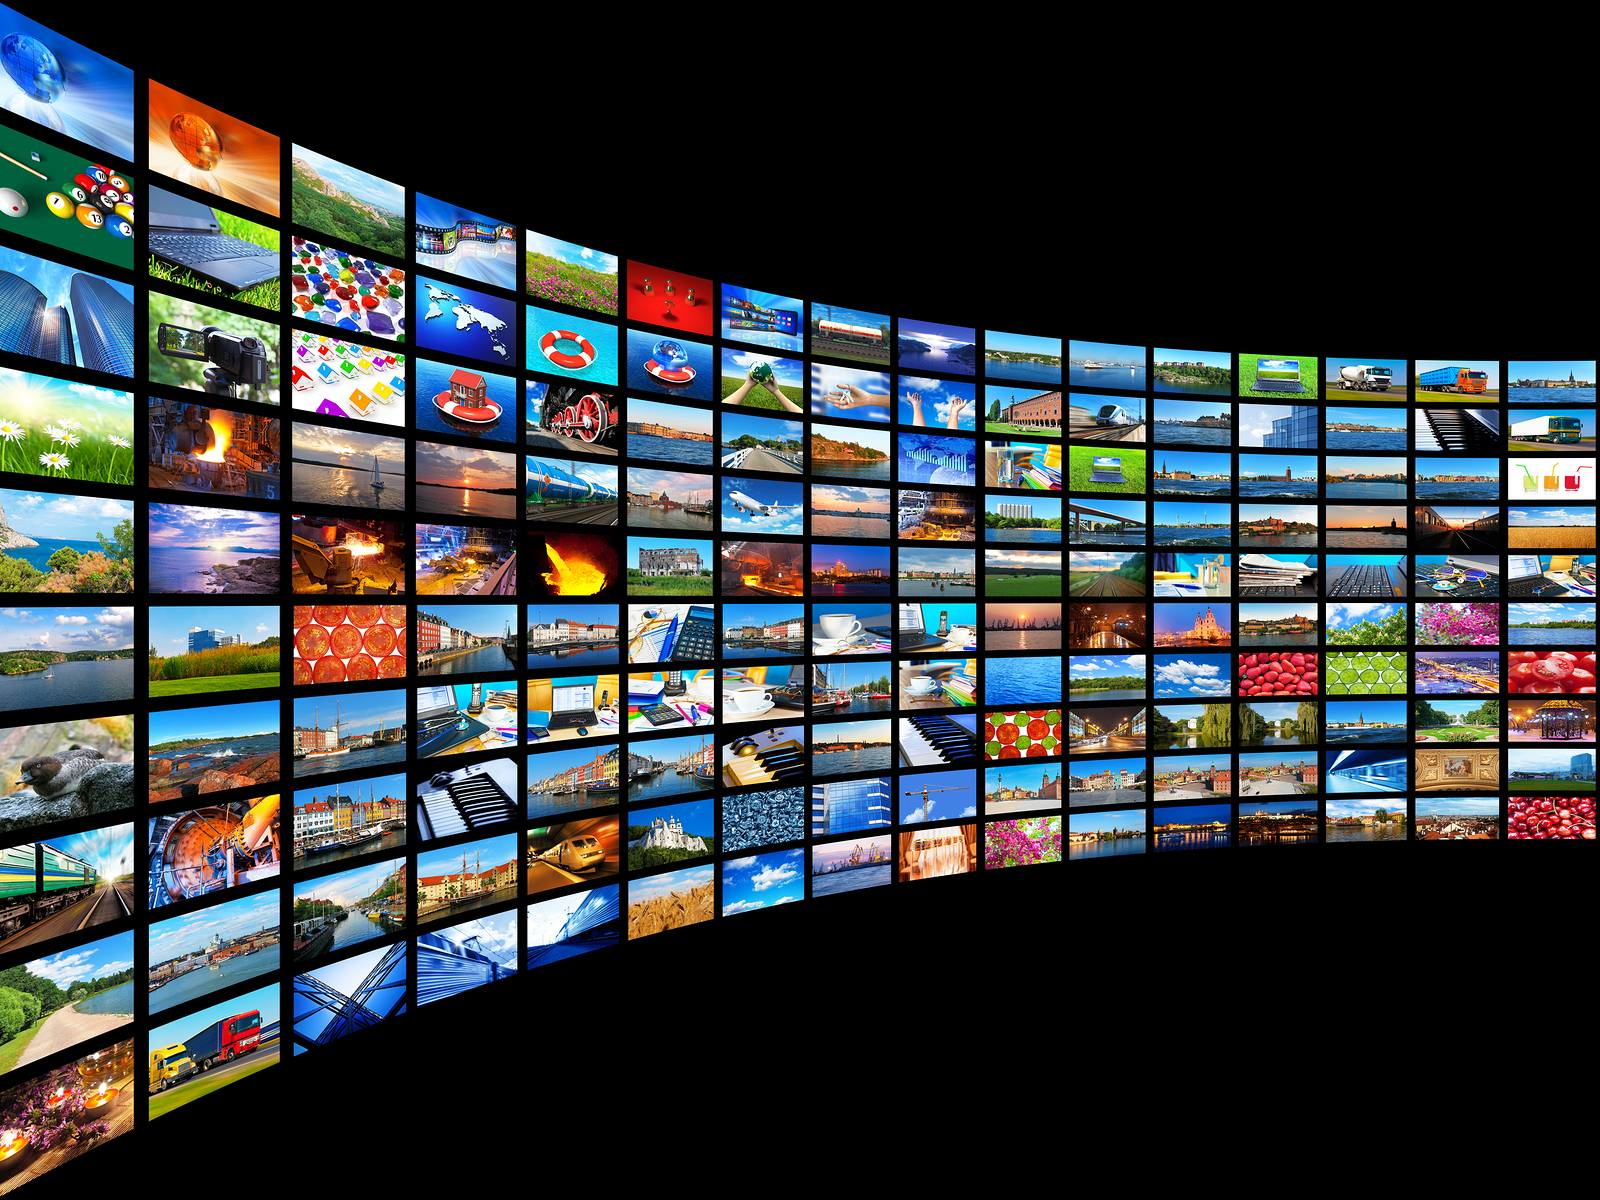
\includegraphics[width=2cm]{medium-video}$\rightarrow 10$
  \end{itemize}
  \bspar1 
  Fragen:
  \begin{itemize}
  \item Welche Arten von Kodierungen kann man Unterscheiden?
  \item Was sind nun effiziente Kodierungen f\"ur verschiedene
    Informationen?
  \item Wieviel Information steckt in einer Nachricht?
  \end{itemize}
\end{bsslide}
%%%%%%%%%%%%%%%%%%%%%%%%%%%%%%%%%%%%%%%%%%%%%%%%%%%%%%%%%%%%%%%%%%%%%%%% 
\renewcommand{\textbufferB}{Kodierung - Bin\"arcodes und das bin\"are Zahlensystem}
\begin{bsslide}
  \bspar1
  \begin{center}
    \vspace{0.4\textheight}
    \large\textbufferB
  \end{center}
\end{bsslide}
%%%%%%%%%%%%%%%%%%%%%%%%%%%%%%%%%%%%%%%%%%%%%%%%%%%%%%%%%%%%%%%%%%%%%%%% 
%%%%%%%%%%%%%%%%%%%%%%%%%%%%%%%%%%%%%%%%%%%%%%%%%%%%%%%%%%%%%%%%%%%%%%%% 
%%%%%%%%%%%%%%%%%%%%%%%%%%%%%%%%%%%%%%%%%%%%%%%%%%%%%%%%%%%%%%%%%%%%%%%% 
%%%%%%%%%%%%%%%%%%%%%%%%%%%%%%%%%%%%%%%%%%%%%%%%%%%%%%%%%%%%%%%%%%%%%%%% 
\begin{bsslide}[\textbufferB]
  \colortext{Motivation}
  \bspar1
  Digitale Ger\"ate basieren auf digitalen Schaltungen welche zwei Zust\"ande unterscheiden k\"onnen:
  \begin{itemize}
  \item Strom Ein (oder $1$)
  \item Strom Aus (oder $0$)
  \end{itemize}
  \bspar1
  Auf digitalen Ger\"aten wird  Information daher als Bin\"arcode repr\"asentiert. Die Digitalisierung kann somit auch als Kodierung eines analogen Signales in einen Bin\"arcode verstanden werden. \\
\end{bsslide}
%%%%%%%%%%%%%%%%%%%%%%%%%%%%%%%%%%%%%%%%%%%%%%%%%%%%%%%%%%%%%%%%%%%%%%%% 
\begin{bsslide}[\textbufferB]
  \colortext{Formale Definition}
  \bspar1
  \begin{definition}[Bin\"arcode]
    Ein Bin\"arcode $c$ ist eine Kodierung, bei dem der
    Ziel-Zeichenvorrat $B$ (die Bildmenge) aus genau zwei Symbolen besteht. Diese werden als Bit (binary digit) bezeichnet.
  \end{definition}
  \bspar3
  \begin{itemize}
  \item Das duales Zahlensystem bestehend aus dem Zeichenvorrat $A=\{0,1\}$ erm\"oglicht arithmethische Operationen im Bin\"arcode
  \item Die Boolesche Algebra (Aussagenlogik), bestehend aus dem Zeichenvorrag $A=\{Wahr,Falsch\}$,  erm\"oglicht logische Operationen 
  \item Alle weiterf\"uhrenden Kodierungen, wie z.B. Zeichens\"atze,
    Audio, Bilder, Videos, Programme etc. werden auf bin\"are Codes zur\"uckgef\"uhrt.
  \end{itemize}
\end{bsslide}

%%%%%%%%%%%%%%%%%%%%%%%%%%%%%%%%%%%%%%%%%%%%%%%%%%%%%%%%%%%%%%%%%%%%%%%% 
\begin{bsslide}[\textbufferB]
  \colortext{Duales Zahlensystem}
  \bspar1
  \textbf{Fragestellung:} Wie sieht ein Bin\"arcode zur Repr\"asentation eines analogen Signals (z.B. Schalldruck) aus, sodass die arithmetische Operationen wie Addition, Subtraktion, Multiplikation erhalten bleiben?

  \bspar2
  Ein solcher Code erm\"oglicht beispielsweise die Addition zweier Signale oder die mathematische Analyse mittels digitalen Ger\"aten (Bild- oder Videobearbeitung, digitale Signalanalyse, Musikkomposition etc.).
\end{bsslide}
%%%%%%%%%%%%%%%%%%%%%%%%%%%%%%%%%%%%%%%%%%%%%%%%%%%%%%%%%%%%%%%%%%%%%%%% 
\begin{bsslide}[\textbufferB]
  \colortext{Duales Zahlensystem - Definition}
  \bspar1
  \textbf{Beobachtung:} Unser dezimales Zahlensystem ist ein Positionssystem mit der \textbf{Basis 10}, in dem eine Zahl in 10er Potenzen zerlegt wird.
  \bspar1
  \begin{definition}[Positionszahlensystem]
    Ein Positionszahlensystem mit der Basis $B$ zerlegt ein Zahl $n=<b_0,b_2,\ldots,b_{N-1}>$ in Ziffern $<b_0,b_2,\ldots,b_{N-1}>$ mit $N$ Stellen aufsteigend geordnet nach Potenzen von B. Der Wert der Zahl $n$ kann als folgende Summe berechnet werden:
    \[
    \sum_{i=0}^{N-1}b_i\cdot B ^i
    \]
    wobei gilt
    \begin{itemize}
    \item $B\in \mathbb{N}$ uynd $B\geq 2$ 
    \item $b_i \in \mathbb{N}_0$, $0\geq b_i< B$
    \end{itemize}
  \end{definition}

\end{bsslide}

%%%%%%%%%%%%%%%%%%%%%%%%%%%%%%%%%%%%%%%%%%%%%%%%%%%%%%%%%%%%%%%%%%%%%%%% 
\begin{bsslide}[\textbufferB]
  \colortext{Duales Zahlensystem - Beispiele}
  \bspar1
  Mit \"Anderung der Basis \"andert sich auch das Zahlensystem und die notwendige Anzahl der Ziffernzeichen:
  \begin{itemize}
  \item Dezimalsystem: $B=10$, Ziffern $0-9$
  \item Bin\"ar- bzw. Dualsystem: $B=2$, Ziffern $\{0,1\}$
  \item Octalsystem: $B=8$, Ziffern $0-7$
  \item Hexadezimalsystem: $B=16$, Ziffern $\{0-9, A, B, C, D, E, F\}$
  \end{itemize}
  \bspar1
  Beispiele: 
  \begin{itemize}
  \item $n_2=1101$\\
    Zahlenwert $n_{10}= 1*2^3+1*2^2+0*2^1+1*2^0=1*8+1*4+0*2+1*1=13$
  \item $n_{16}=BAB$\\
    Zahlenwert $n_{10}= 11*16^2+10*16^1+11*16^0=11*256+10*16+11*1 = 2987$
  \item $n_{8}=3110$\\ 
    Zahlenwert $n_{10}= 3*8^3+1*8^2+1*8^1+0*8^0=1608$
  \end{itemize}
\end{bsslide}
%%%%%%%%%%%%%%%%%%%%%%%%%%%%%%%%%%%%%%%%%%%%%%%%%%%%%%%%%%%%%%%%%%%%%%%% 
\begin{bsslide}[\textbufferB]
  \colortext{Duales Zahlensystem - Hex, Octal und Bin\"ar}
  \bspar1\small
  Das Hexadezimal- und Oktalsystem stellen eine k\"urzere, einfach ermittelbare Schreibweise zum Bin\"arsystem dar, da ihre Basen Potenzen von 2 darstellen. Eine Umrechnung ist einfach m\"oglich, da Hexadezimalzahlen durch 4 Bit und Oktalzahlen durch 3 Bit repr\"asentiert werden k\"onnen:
  \bspar1
  \begin{center}
    \begin{tabular}{lcccc}
      \textbf{$n_{10}$}   &   \textbf{$n_2$}     & \textbf{$n_{8}$}    & \textbf{$n_{16}$}  \\
      \hline
      0  &      $0000$          &      $0$      &      $0$     \\
      1  &      $0001$          &      $1$      &      $1$     \\
      2  &      $0010$          &      $2$      &      $2$     \\
      3  &      $0011$          &      $3$      &      $3$     \\
      4  &      $0100$          &      $4$      &      $4$     \\
      5  &      $0101$          &      $5$      &      $5$     \\
      6  &      $0110$          &      $6$      &      $6$     \\
      7  &      $0111$          &      $7$      &      $7$     \\
      8  &      $1000$          &      $10$      &      $8$     \\
      9  &      $1001$          &      $11$      &      $9$     \\
      10  &      $1010$          &      $12$      &      $A$     \\
      11  &      $1011$          &      $13$      &      $B$     \\
      12  &      $1100$          &      $14$      &      $C$     \\
      13  &      $1101$          &      $15$      &      $D$     \\
      14  &      $1110$          &      $16$      &      $E$     \\
      15  &      $1111$          &      $17$      &      $F$     \\
      \hline
    \end{tabular}
  \end{center}
\end{bsslide}
%%%%%%%%%%%%%%%%%%%%%%%%%%%%%%%%%%%%%%%%%%%%%%%%%%%%%%%%%%%%%%%%%%%%%%%% 
\begin{bsslide}[\textbufferB]
  \colortext{Duales Zahlensystem - Umwandlung aus dem Dezimalsystem}
  \bspar1
  F\"ur die Umwandlung einer Dezimalzahl $x$ in ein Zahlensystem mit der Basis $B$ kann folgender Algorithmus verwendet werden:
  \begin{enumerate}
  \item Division durch Basis: $\frac{x}{B} = y\;Rest\;z$
  \item Mache $y$ zum neuen $x$
  \item Solange $x$ ungleich 0 gehe zu Schritt 1
  \item Die ermittelten Reste $z$ von unten nach oben nebeneinander (von links nach rechts) geschrieben ergeben die entsprechende Zahl zur Basis $B$
  \end{enumerate}
  \bspar1
  \textbf{Warum?}
  \bspar1
  Laut Hornerschema kann ein Zahl zur Basis $B$ wie folgt zerlegt werden:
  \[
  \sum_{i=0}^{N-1}b_i\cdot B ^i = (\ldots(((b_N*B_N+b_{N-1})*B+b_{N-2})*B+\ldots+b_1)*B+b_0
  \]

  Eine Division der obigen Summe durch $B$ ergibt:\\
  $
  y = (\ldots(((b_N*B_N+b_{N-1})*B+b_{N-2})*B+\ldots+b_1)
  $
  und 
  $
  z = b_0
  $
\end{bsslide}
%%%%%%%%%%%%%%%%%%%%%%%%%%%%%%%%%%%%%%%%%%%%%%%%%%%%%%%%%%%%%%%%%%%%%%%% 
\begin{bsslide}[\textbufferB]
  \colortext{Duales Zahlensystem - Umwandlung aus dem Dezimalsystem}
  \bspar1
  Beispiel: $n_{10}=68$ im Dualsystem?
  \begin{center}
    \begin{tabular}{ccc}
      \textbf{$x$}   &   \textbf{$y$}     & \textbf{$z$}  \\
      \hline
      68  &     34 &  0       \\
      34  &     17 & 0       \\
      17  &     8   & 1       \\
      8  &     4   & 0       \\
      4  &     2   & 0       \\
      2 &      2  & 0\\
      1 &      2  & 1\\
      0 &      -  & -\\
      \hline
    \end{tabular}
  \end{center}
  $n_{10}=68\rightarrow n_2=1000100$ 
\end{bsslide}

%%%%%%%%%%%%%%%%%%%%%%%%%%%%%%%%%%%%%%%%%%%%%%%%%%%%%%%%%%%%%%%%%%%%%%%% 
\renewcommand{\textbufferB}{Kodierung - Rechnen im  bin\"aren Zahlensystem}
\begin{bsslide}
  \bspar1
  \begin{center}
    \vspace{0.4\textheight}
    \large\textbufferB
  \end{center}
\end{bsslide}
%%%%%%%%%%%%%%%%%%%%%%%%%%%%%%%%%%%%%%%%%%%%%%%%%%%%%%%%%%%%%%%%%%%%%%%% 
%%%%%%%%%%%%%%%%%%%%%%%%%%%%%%%%%%%%%%%%%%%%%%%%%%%%%%%%%%%%%%%%%%%%%%%% 
%%%%%%%%%%%%%%%%%%%%%%%%%%%%%%%%%%%%%%%%%%%%%%%%%%%%%%%%%%%%%%%%%%%%%%%% 
%%%%%%%%%%%%%%%%%%%%%%%%%%%%%%%%%%%%%%%%%%%%%%%%%%%%%%%%%%%%%%%%%%%%%%%% 
\begin{bsslide}[\textbufferB]
  \colortext{Arithmetische Operationen}
  \bspar1
  Das bin\"are Zahlensystem erlaubt alle arithmetischen Operationen und ist somit \"aquivalent zum Dezimalsystem. Es gelten die gleichen Rechenregeln:
  \begin{center}
    \begin{tabular}{cc|c|c|c|c|}
      \textbf{$x$}   &   \textbf{$y$}     & \textbf{$x+y$} & \textbf{$x-y$}& \textbf{$x*y$}& \textbf{$x/y$}  \\
      \hline
      0    & 0 & 0 & 0 & 0 & not defined (n.d.) \\
      0    & 1 & 1 & -1 bzw. 11\footnote{In B-Komplementdarstellung, siehe n\"achsten Folien} & 0 & 0\\
      1    & 0 & 1 & 1 & 0 & not defined (n.d.) \\
      1    & 1 & 10 & 0 & 1 & 1  \\
      \hline
    \end{tabular}
  \end{center}
\bspar1\tiny
Bei der Subtraktion entspricht  11 der  B-Komplementdarstellung, die
auf den n\"achsten Folien erkl\"art wird.
\end{bsslide}

%%%%%%%%%%%%%%%%%%%%%%%%%%%%%%%%%%%%%%%%%%%%%%%%%%%%%%%%%%%%%%%%%%%%%%%% 
\begin{bsslide}[\textbufferB]
  \colortext{Arithmetische Operationen}
  \bspar1
  Beispiel Addition mehrstelliger Zahlen:
  \bspar3
  \begin{center}
    \begin{tabular}{lrr}
      {x} &                10011011 & (155) \\
      {y} &                00111110 & (62)\\
      \hline
      {\"Ubertrag} & 01111100 &\\
      \hline
      {Ergebnis} &    11011001& (217)\\   
    \end{tabular}
  \end{center}
  Wichtig: der \"Ubertrag erfolgt immer wenn die Summe gr\"o\ss er 1 wird
\end{bsslide}

%%%%%%%%%%%%%%%%%%%%%%%%%%%%%%%%%%%%%%%%%%%%%%%%%%%%%%%%%%%%%%%%%%%%%%%% 
\begin{bsslide}[\textbufferB]
  \colortext{Arithmetische Operationen}
  \bspar1
  \textbf{Zur Subtraktion} m\"ussen wir noch \"uberlegen, wie negative Zahlen dargestellt werden k\"onnen. Im Normalfall werden negative Zahlen durch ihren Betrag mit vorangestellten Minus dargestellt, worauf ein Bit verwendet werden k\"onnte. Um jedoch die Subtraktion rechnerisch mittels Addition abzubilden (und somit die Rechnerarchitektur zu vereinfachen), wird auf die so genannten \textbf{Zweierkomplementdarstellung} zur\"uckgegriffen. 
  \bspar1
  In der Zweierkomplementdarstellung (oder auch B-Komplement
  darstellung wobei B die Basis, im dual System also 2, angibt) werden negative Zahlen durch ein auf 1 gesetztes f\"uhrendes Bit dargestellt. Die positiven Zahlen inklusive $0$ werden durch ein auf $0$ gesetztes f\"uhrendes Bit dargestellt. 
  \bspar1
\end{bsslide}

\begin{bsslide}[\textbufferB]
  \colortext{Arithmetische Operationen}
  \bspar1
  Zweierkomplement: Beispiel mit drei Bit:
  \begin{center}
    \begin{tabular}{lcccc}
      \textbf{Dezimal}   &   \textbf{B-Komplement}     & \textbf{mit Vorzeichen Bit}  \\
      -4  &     100  &   NA       \\
      -3  &     101  &    111      \\
      -2  &     110  &    110       \\
      -1  &     111  &    101       \\
      0 &     000  &    000 od. 100      \\
      1 &     001  &    001       \\
      2 &     010  &    010      \\
      3 &     011  &    011  \\
      \hline
    \end{tabular}
  \end{center}
  Wie erkennbar ``verschwendet'' das Vorzeichenbit zwei Bin\"aerzahlen zur Kodierung der 0.
\end{bsslide}

%%%%%%%%%%%%%%%%%%%%%%%%%%%%%%%%%%%%%%%%%%%%%%%%%%%%%%%%%%%%%%%%%%%%%%%% 
\begin{bsslide}[\textbufferB]
  \colortext{Arithmetische Operationen}
  \bspar1
  Das Zweierkomplement wird wie folgt erzeugt:
  \begin{enumerate}
  \item Konvertiere die Zahl ohne Vorzeichen in das Bin\"arsystem
  \item Invertiere die Bits der konvertierten Zahl
  \item Addiere 1 zur invertierten Zahl.
  \end{enumerate}
  \bspar1
  Beispiel f\"ur -5:
  \begin{center}
    \begin{tabular}{lr}
      {Umwandeln} & 0101     \\
      {Invertieren} &  1010 \\
      {+1} & 1011 \\    
    \end{tabular}
  \end{center}
\end{bsslide}
%%%%%%%%%%%%%%%%%%%%%%%%%%%%%%%%%%%%%%%%%%%%%%%%%%%%%%%%%%%%%%%%%%%%%%%% 
\begin{bsslide}[\textbufferB]
  \colortext{Arithmetische Operationen}
  \bspar1
  Beispiel Subtraktion mehrstelliger Zahlen: 155-62.
  \bspar1
  \begin {enumerate}
  \item Wir rechnen 155 + (-62).
    \bspar1
  \item     Zweierkomplementdarstellung von 62:
    \begin{center}
      \begin{tabular}{lr}
        {Umwandeln} & 000111110     \\
        {Invertieren} &  111000001 \\
        {+1} &              111000010 \\
      \end{tabular}
    \end{center}
    \bspar1
  \item Durchf\"uhren der Addition:
    \begin{center}
      \begin{tabular}{lrr}
        {x} &                010011011 & (155) \\
        {y} &                111000010 & (-62)\\
        {\"Ubertrag} & 100000100& {Das f\"uhrende \"Ubertragsbit wird verworfen}\\
        \hline
        {Ergebnis} &    001011101&  (93)\\   
      \end{tabular}
    \end{center}
  \end {enumerate}
\end{bsslide}


%%%%%%%%%%%%%%%%%%%%%%%%%%%%%%%%%%%%%%%%%%%%%%%%%%%%%%%%%%%%%%%%%%%%%%%% 
\renewcommand{\textbufferB}{Kodierung - ASCII Code}
\begin{bsslide}
  \bspar1
  \begin{center}
    \vspace{0.4\textheight}
    \large\textbufferB
  \end{center}
\end{bsslide}
%%%%%%%%%%%%%%%%%%%%%%%%%%%%%%%%%%%%%%%%%%%%%%%%%%%%%%%%%%%%%%%%%%%%%%%% 
\begin{bsslide}[\textbufferB]
  \colortext{ASCII Code}
  \bspar1
   Eine ander Art der Kodierung sind Zeichensatzkodierungen, wie der
   \textbf{American Standard Code for Information Interchange (kurz
     ASCII Code).} 
\bspar1
   Der Zeichensatz kodiert mit 7-Bit das lateinische Alphabet in
   Gro\ss- und Kleinschreibung, die arabischen Ziffern sowie
   Satzzeichen und Sonderzeichen. Er beinhaltet alle wesentlichen Zeichen einer Tastatur. 
\bspar1
   Jedem Zeichen des Zeichensatzes wird dabei ein
   Bin\"arcode per Definition zugewiesen. D.h. es gibt 128
   verschiedene Bitmuster.
\end{bsslide}


\begin{bsslide}[\textbufferB]
  \colortext{ASCII Code}
  \bspar1
  \bsfigurecaption[0.8]{asciifull}{\tiny Bildquelle \url{http://www.asciitable.com/}}
\end{bsslide}
%%%%%%%%%%%%%%%%%%%%%%%%%%%%%%%%%%%%%%%%%%%%%%%%%%%%%%%%%%%%%%%%%%%%%%%% 
%%%%%%%%%%%%%%%%%%%%%%%%%%%%%%%%%%%%%%%%%%%%%%%%%%%%%%%%%%%%%%%%%%%%%%%%
%%%%%%%%%%%%%%%%%%%%%%%%%%%%%%%%%%%%%%%%%%%%%%%%%%%%%%%%%%%%%%%%%%%%%%%%
\renewcommand{\textbufferB}{Kodierung -Zusammenfassung}
\begin{bsslide}
  \bspar1
  \begin{center}
 \vspace{0.4\textheight}
    \large\textbufferB
  \end{center}
\end{bsslide}
%%%%%%%%%%%%%%%%%%%%%%%%%%%%%%%%%%%%%%%%%%%%%%%%%%%%%%%%%%%%%%%%%%%%%%%%
%%%%%%%%%%%%%%%%%%%%%%%%%%%%%%%%%%%%%%%%%%%%%%%%%%%%%%%%%%%%%%%%%%%%%%%%
%%%%%%%%%%%%%%%%%%%%%%%%%%%%%%%%%%%%%%%%%%%%%%%%%%%%%%%%%%%%%%%%%%%%%%%%
%%%%%%%%%%%%%%%%%%%%%%%%%%%%%%%%%%%%%%%%%%%%%%%%%%%%%%%%%%%%%%%%%%%%%%%%
%%%%%%%%%%%%%%%%%%%%%%%%%%%%%%%%%%%%%%%%%%%%%%%%%%%%%%%%%%%%%%%%%%%%%%%%
\begin{bsslide}[Zusammenfassung]
  \colortext{Kodierung}
  \bspar1
  \begin{itemize}	
  \item Repr\"asentation von Information mittels Zeichen und Nachrichten
  \item Kodierung als Vorschrift zur \"Uberf\"uhrung Nachrichten
    aus einem Zeichensatz in den anderen. 
  \item Bin\"arcodes bestehen aus genau zwei Zeichen, welche
    unterschiedliche interpretiert werden k\"onnen:
    \begin{itemize}
    \item Als Zahl im dualen Zahlensystem
      \begin{itemize}
      \item Positionszahlensystem zur Basis 2
      \item Arithmetische Operationen
      \item Subtraktion als Addition mittels Zweierkomplement
      \end{itemize}
    \item Als Zeichen einer Tastatur (ASCII Code)
    \item Als Wahrheitswerte (Wahr/Falsch) im Bereich der Aussagenlogik
    \end{itemize}
  \end{itemize}
\end{bsslide}
%%%%%%%%%%%%%%%%%%%%%%%%%%%%%%%%%%%%%%%%%%%%%%%%%%%%%%%%%%%%%%%%%%%%%%%%
%%%%%%%%%%%%%%%%%%%%%%%%%%%%%%%%%%%%%%%%%%%%%%%%%%%%%%%%%%%%%%%%%%%%%%%%
\begin{bsslide}[Bibliographie]
  \bspar4
  \begin{itemize}
  \item \textbf{Malaka, Butz, Hussmann (2009)} -
    Medieninformatik: Eine Einf\"uhrung (Pearson Studium - IT), Kapitel
    2.4
 \item \textbf{Herold, Lurz, Wohlrab} - Grundlagen der Informatik,
   Pearson Studium, Kapitel 3
  \end{itemize}
\end{bsslide}
 

\outline
%%% DATE.  November, 17th, 2013

\clearpage

%%%%%%%%%%%%%%% METADATA %%%%%%%%%%%%%%%%
\bsunitname{Informationstheorie}
\setcounter{bsunit}{3}
%%%%%%%%%%%%%%%%%%%%%%%%%%%%%%%%%%%%%%%%%%%%%%%%%%%%%%%%%%%%%%%%%%%%%%%%
%%% SOURCE. \cf[Kapitel 2]{Malak, Butz, Hu�mann - Einf�hrung Medieninformatik}
%%%%%%%%%%%%%%%%%%%%%%%%%%%%%%%%%%%%%%%%%%%%%%%%%%%%%%%%%%%%%%%%%%%%%%%%
\renewcommand{\textbufferB}{Informationstheorie - Ein einf\"uhrendes Beispiel}
\begin{bsslide}
  \bspar1
  \begin{center}
 \vspace{0.4\textheight}
    \large\textbufferB
  \end{center}
\end{bsslide}
%%%%%%%%%%%%%%%%%%%%%%%%%%%%%%%%%%%%%%%%%%%%%%%%%%%%%%%%%%%%%%%%%%%%%%%%
\begin{bsslide}[\textbufferB]
  \colortext{Problemstellung}
  \bspar1
  Wir haben unterschiedliche Kodierungen mit verschiedenen
  Eigenschaften kennen gelernt.
  \bspar2
  Doch wann ist eine Kodierung optimial, d.h. existiert eine Kodierung die mit
  weniger Bit die gleiche Information \"ubermitteln kann?
  \bspar2
  Wie kann man die Menge der in einer Nachricht erhaltenen Information
  quantifizieren?
  \bspar2
  Wie kann man den Informationsgehalt einer Nachrichtenquellen quantifizieren?
\end{bsslide}
%%%%%%%%%%%%%%%%%%%%%%%%%%%%%%%%%%%%%%%%%%%%%%%%%%%%%%%%%%%%%%%%%%%%%%%%
\renewcommand{\textbufferA}{\bspar1
  Nehmen wir an sie haben ein Kartenspiel bestehend aus 4 Karten,
  $K=\{1,2,3,4\}$.  Person A zieht eine Karte. Person B muss \"uber
  m\"oglichst wenige ``Ja/Nein'' Antworten herausfinden, um welche
  Karte es sich handelt.}
\begin{bsslide}[\textbufferB]
  \colortext{Beispiel Kartenspiel}
  \textbufferA
\end{bsslide}
%%%%%%%%%%%%%%%%%%%%%%%%%%%%%%%%%%%%%%%%%%%%%%%%%%%%%%%%%%%%%%%%%%%%%%%%
\begin{bsslide}[\textbufferB]
  \colortext{Beispiel Kartenspiel}
  \textbufferA
  \bspar1
   \bsfigurecaption[1.0]{Codierungstheorie-Beispiel-Code-A}{Beispiel Fragebaum A}
\end{bsslide}
%%%%%%%%%%%%%%%%%%%%%%%%%%%%%%%%%%%%%%%%%%%%%%%%%%%%%%%%%%%%%%%%%%%%%%%%
\begin{bsslide}[\textbufferB]
  \colortext{Beispiel Kartenspiel}
  \textbufferA
  \bspar1
   \bsfigurecaption[1.0]{Codierungstheorie-Beispiel-Code-B}{Beispiel Fragebaum B}
\end{bsslide}
%%%%%%%%%%%%%%%%%%%%%%%%%%%%%%%%%%%%%%%%%%%%%%%%%%%%%%%%%%%%%%%%%%%%%%%%
\begin{bsslide}[\textbufferB]
  \colortext{Beispiel Kartenspiel}
\bspar1
  Jede ``Ja/Nein'' Antwort kann als Bit (``0/1'') verstanden werden,
  wodurch sich folgender Bin\"arcode ergibt:
  \begin{center}
    \begin{tabular}{lrrc}
      \textbf{Karte} &\textbf{Code A} &\textbf{Code B} &\textbf{Informationsgehalt}\\
      \hline
      1                    &                          1&   00  & 2\\
      2                    &                        10&   01  & 2\\
      3                    &                      100&   10  & 2\\
      4                    &                    1000&   11  & 2\\
    \end{tabular}
  \end{center}
  \bspar1
  Beobachtungen:
  \begin{itemize}
  \item  Code B scheint effizienter, da er im Schnitt weniger Fragen (Bits)
    ben\"otigt.
  \item  Code B scheint optimal zu sein, da wir f\"ur 4 Zust\"ande 2
    Bits ben\"otigen ($N = 2^{\#bits}$ bzw. $\#bits = \log_2 (N)$ mit $N$
    als Anzahl der Karten)
  \item Alternativ: In Code B reduziert jede Frage die Unsicherheit um 50 \%
    d.h. die Anzahl der verbleibenden M\"oglichkeiten wird um die
    H\"alfte reduziert
  \item Der Informationsgehalt einer Karte kann als minimale
    Anzahl von  Ja/Nein Fragen aufgefasst werden.
  \end{itemize}
\end{bsslide}
%%%%%%%%%%%%%%%%%%%%%%%%%%%%%%%%%%%%%%%%%%%%%%%%%%%%%%%%%%%%%%%%%%%%%%%%
\renewcommand{\textbufferA}{\bspar1
  Ein neues Spiel hat folgende 4 Karten: $K=\{1,1,2,3\}$, d.h. Karte 1
  kommt 2x vor. Wie \"andert sich der Code?}
%%%%%%%%%%%%%%%%%%%%%%%%%%%%%%%%%%%%%%%%%%%%%%%%%%%%%%%%%%%%%%%%%%%%%%%%
\begin{bsslide}[\textbufferB]
  \colortext{Beispiel Kartenspiel}
  \textbufferA
\end{bsslide}
%%%%%%%%%%%%%%%%%%%%%%%%%%%%%%%%%%%%%%%%%%%%%%%%%%%%%%%%%%%%%%%%%%%%%%%%
\renewcommand{\textbufferA}{\bspar1
  Ein neues Spiel hat folgende 4 Karten: $K=\{1,1,2,3\}$, d.h. Karte 1
  kommt 2x vor.
  \begin{center}
    \begin{tabular}{lrrc}
      \textbf{Karte} &\textbf{Code B} &\textbf{Code C}  &\textbf{Informationsgehalt}\\
      \hline
      1                    &                    00&   0  & 1\\
      1                    &                    01&   0  & 1\\
      3                    &                    10&   01  & 2\\
      4                    &                    11&   11  & 2\\
    \end{tabular}
  \end{center}}
%%%%%%%%%%%%%%%%%%%%%%%%%%%%%%%%%%%%%%%%%%%%%%%%%%%%%%%%%%%%%%%%%%%%%%%%
\begin{bsslide}[\textbufferB]
  \colortext{Beispiel Kartenspiel}
  \textbufferA
  \bspar1
  \textbf{Fragen}:
  \begin{itemize}
  \item \textbf{Bit 0}: Ist es nicht 1?
  \item \textbf{Bit 1}: Ist es 4?
    \end{itemize}
  Der Code ist optimal, da beide Fragen die Unsicherheit um 50\%
  reduzieren, d.h. die Anzahl der verbleibenden M\"oglichkeiten auf
  die H\"alfte reduzieren.
\end{bsslide}
%%%%%%%%%%%%%%%%%%%%%%%%%%%%%%%%%%%%%%%%%%%%%%%%%%%%%%%%%%%%%%%%%%%%%%%%
\begin{bsslide}[\textbufferB]
  \colortext{Beispiel Kartenspiel}
  \textbufferA
  \bspar1
  \textbf{Beobachtungen}:
  \begin{itemize}
  \item  Code C scheint effizienter, da er im Schnitt weniger Fragen (Bits)
    ben\"otigt.
  \item 2 Karten haben dieselbe Bedeutung.
    \begin{itemize}
    \item Da es wahrscheinlicher
    ist, Karte 1 zu ziehen, ist der Informationsgehalt von Karte 1
    jedoch geringer.
    \item Alternativ: Da Karte 1 \"ofters gezogen wird, wollen wir der
      Karte einen k\"urzeren Code geben.
 \end{itemize}
 \end{itemize}
\end{bsslide}
%%%%%%%%%%%%%%%%%%%%%%%%%%%%%%%%%%%%%%%%%%%%%%%%%%%%%%%%%%%%%%%%%%%%%%%%
\begin{bsslide}[\textbufferB]
  \colortext{Beispiel Kartenspiel}
  \textbufferA
  \bspar1
  Wie hoch ist der Informationsgehalt von Karte 1?
  \begin{itemize}
  \item F\"ur 4 Karten benotigen wir 2 bit ($\log_2 (4)$).
  \item Karte 1 w\"urde dabei 2 Codes erhalten, die jedoch  die
    gleiche Bedeutung haben und somit redundant sind. D.h. 1 Frage/Bit ($\log_2(2)$) ist redundant.
  \item $IG(Karte_1) = \log_2 (4)-\log_2 (2)=\log_2 (\frac{4}{2})=\log_2
    (\frac{1}{p(Karte_1)})$\\
    wobei $p(Karte_1)$ die Wahrscheinlichkeit darstellt, dass $Karte_1$
    gezogen wird.
\item Analog f. Karte 3: $IG(Karte_3) = \log_2 (4)-\log_2 (1)=\log_2 (\frac{4}{1})=\log_2
    (\frac{1}{p(Karte_3)})$
  \end{itemize}
\end{bsslide}
%%%%%%%%%%%%%%%%%%%%%%%%%%%%%%%%%%%%%%%%%%%%%%%%%%%%%%%%%%%%%%%%%%%%%%%%
\renewcommand{\textbufferA}{\bspar1
  Nehmen wir an sie haben ein Kartenspiel bestehend aus 4 Karten,
  $K=\{1,2,3,4\}$.  Person A zieht eine Karte. Person B muss \"uber
  m\"oglichst wenige ``Ja/Nein'' Antworten herausfinden, um welche
  Karte es sich handelt.}

%%%%%%%%%%%%%%%%%%%%%%%%%%%%%%%%%%%%%%%%%%%%%%%%%%%%%%%%%%%%%%%%%%%%%%%%
\renewcommand{\textbufferB}{Informationstheorie - Formale Definition}
\begin{bsslide}
  \bspar1
  \begin{center}
 \vspace{0.4\textheight}
    \large\textbufferB
  \end{center}
\end{bsslide}
%%%%%%%%%%%%%%%%%%%%%%%%%%%%%%%%%%%%%%%%%%%%%%%%%%%%%%%%%%%%%%%%%%%%%%%%
\begin{bsslide}[\textbufferB]
  \colortext{�berblick}
  \bspar1
  \begin{itemize}
  \item Die Informationstheorie nach Shannon wurde 1948 von \textbf{Claude
      Shannon} entwickelt.
  \item Sie stellt ein \textbf{mathematisches Modell} f\"ur
    Kommunikationssysteme dar.
  \item  Dabei werden Nachrichten als
    \textbf{stochastische Ereignisse}, die von einer
    Nachrichtenquelle, dem Sender, ausgesendet und von einem
    Empf\"anger empfangen werden. \\[-1ex]
    \begin{itemize}
    \item Stochastische Prozesse sind zeitlich geordnete, zuf�llige
      Prozesse die mit Hilfe der Statistik und
      Wahrscheinlichkeitsrechnung beschrieben werden
    \item Nachrichten bestehen somit aus einer endlichen Anzahl
      diskreter Zeichen, welche mit einer
      gewissen Wahrscheinlichkeit auftreten.
    \end{itemize}
  \end{itemize}
\end{bsslide}
%%%%%%%%%%%%%%%%%%%%%%%%%%%%%%%%%%%%%%%%%%%%%%%%%%%%%%%%%%%%%%%%%%%%%%%%
\begin{bsslide}[\textbufferB]
  \colortext{�berblick}
  \bspar1
  Kernelemente der Informationstheorie:
  \begin{itemize}
  \item Definition einer \textbf{Nachrichtenquellen} und deren Eigenschaften
  \item Definition des \textbf{Informationsgehaltes bzw. der Information eines Zeichens, $I(x)$}
  \item Definition der \textbf{Entropie $H(X)$}, d.h. der Informationsdichte bzw. des
    durchschnittlichen Informationsgehaltes einer Nachrichtenquelle
   \item Definition von \textbf{optimalen Kodierungen }und darauf aufbauender \textbf{Redundanz}
  \end{itemize}
\end{bsslide}

%%%%%%%%%%%%%%%%%%%%%%%%%%%%%%%%%%%%%%%%%%%%%%%%%%%%%%%%%%%%%%%%%%%%%%%%
  \begin{bsslide}[\textbufferB]
    \colortext{Nachrichtenquelle}
    \bspar1
    \begin{definition}[Diskrete, ged\"achtnislose Nachrichtenquelle]
      Eine diskrete, ged\"achtnislose Nachrichtenquelle setzt in jedem
      Zeittakt ein Zeichen $a_i \in A$ aus einem Zeichenvorrat $A$ mit
      der Wahrscheinlicheit $P(a_i)=p_i$ ab. Die Auswahl der Zeichen
      ist unabh\"angig von bereits emitierten Zeichen in der Vergangenheit.
    \end{definition}
    \bspar1
    Beispiel mit 3 Quellen, Zeichenvorrat $\{A,B,C,D\}$:
      \begin{center}
      \begin{tabular}{|l|c|c|c|c|}
        \hline
        Zeichen $a$  	&  A 	& B		& C		&D		\\
\hline
Wahrscheinlichkeit $p_a$ in Quelle 1 & 1.0 & 0.0 & 0.0 & 0.0 \\
Wahrscheinlichkeit $p_a$ in Quelle 2 & 0.25 & 0.25 & 0.25 & 0.25 \\
Wahrscheinlichkeit $p_a$ in Quelle 3 & 0.5 & 0.25 & 0.125 & 0.125 \\
\hline
      \end{tabular}
    \end{center}
      \bspar1
      \begin{itemize}
      \item Welche Quelle �bertr�gt die meiste Information in einer
        Nachricht?
      \item  Wieviel Bit ben�tigen wir zur Kodierung eines Zeichens einer
        Quelle?
       \item Wie hoch ist die Information (bzw. der
         Informationsgehalt) eines Zeichens?
      \end{itemize}
  \end{bsslide}
 %%%%%%%%%%%%%%%%%%%%%%%%%%%%%%%%%%%%%%%%%%%%%%%%%%%%%%%%%%%%%%%%%%%%%%%%
  \begin{bsslide}[\textbufferB]
    \colortext{Informationsgehalt eines Zeichen}
    \bspar1
    \textbf{Axiomatische Definition}\footnote{Axiome sind die Grunds\"atze
      bzw. fixen Annahmen einer Theorie. In einer Axiomatisch
      Definition werden dies a-priori festgelegt. Aus den Axiomen
      werden anschlie\ss end deduktiv weitere Eigenschaften
      abgeleitet.} des Informationsgehalts \"uber 3 Axiome
    (grunds\"atzliche Eigenschaften):
    \begin{enumerate}
    \item[(I)] Der Informationsgehalt eines Zeichens $a\in A$ mit der
      Wahrscheinlicheit $p_i$ ist ein nicht-negatives Ma\ss, welches nur
      von der Wahrscheinlichkeit des Zeichens abh\"angt: $I(p_i)\geq
      0$
     \item[(II)] Der Informationsgehalt zweier voneinander unabh\"angiger
       Zeichen $a_i$ und $a_j$ mit den Wahrscheinlichkeiten $p_i$ und
       $p_j$ addiert sich: $I(p_i, p_j)=I(p_i) + I (p_j)$
     \item[(III)] Der Informationsgehalt ist eine stetige Funktion der
       Wahrscheinlichkeiten der Zeichen.
    \end{enumerate}
  \end{bsslide}

 %%%%%%%%%%%%%%%%%%%%%%%%%%%%%%%%%%%%%%%%%%%%%%%%%%%%%%%%%%%%%%%%%%%%%%%%
\renewcommand{\textbufferA}{\bspar1
    \begin{theorem}[Informationsgehalt/Entscheidungsgehalt eines Zeichens]
    Sei $p_i$ die Wahrscheinlichkeit f�r das Auftreten von Zeichen $a_i\in A$. Der Entscheidungsgehalt $x_i$  f�r das Zeichen $a_i\in A$ ist definiert als
      \[2^{x_a}=1/p_a \Rightarrow x_a = \log_2(1/p_a)\]
    Die Einheit ist bit (basic indissoluble\footnote{unaufl�slich} information unit) pro Zeichen. n bit entsprechen dabei mindestens n Bit (Binary Digits)
    \end{theorem}}

 \begin{bsslide}[\textbufferB]
    \colortext{Informationsgehalt eines Zeichen}
    \textbufferA
    \bspar1
     \begin{center}
      \begin{tabular}{|l|c|c|c|c|}
        \hline
        Zeichen $a$  	&  A 	& B		& C		&D		\\
\hline
$p_a$ in Quelle 1 & 1.0 & 0.0 & 0.0 & 0.0 \\
$x_a$ (in bit) in Quelle 1 & 0 & undef. & undef. & undef. \\
\hline
$p_a$ in Quelle 2 & 0.25 & 0.25 & 0.25 & 0.25 \\
$x_a$ (in bit)in Quelle 2 & 2 & 2 & 2 & 2 \\
\hline
$p_a$ in Quelle 3 & 0.5 & 0.25 & 0.125 & 0.125 \\
$x_a$ (in bit)in Quelle  & 1 & 2 & 3 & 3 \\
\hline
      \end{tabular}
     \end{center}
  \end{bsslide}
%%%%%%%%%%%%%%%%%%%%%%%%%%%%%%%%%%%%%%%%%%%%%%%%%%%%%%%%%%%%%%%%%%%%%%%%
 \begin{bsslide}[\textbufferB]
    \colortext{Informationsgehalt eines Zeichen}
    \textbufferA
    \bspar1\small
    \textbf{Eigenschaften:}
    \begin{itemize}
    \item Ein sicheres Ereignis ($p_i=1.0$) besitzt keine Information.
    \item Unwahrscheinliche Ereignisse besitzen viel Information.
    \item Der Informationsgehalt spiegelt die Axiome wider, wobei der
      Logarithmus f\"ur die Additivit\"at (Axiom II) sorgt
    \item Die Basis des Logarithmus definiert die Einheit. Bei einem
      $\log_{10}$ w\"uerden Zeichen in einem Dezimalcode kodiert
      werden.
   \item Ein bit definiert die kleinste Einheit und kann als
     ``Ja/Nein'' Entscheidung verstanden werden.

    \end{itemize}
  \end{bsslide}
 %%%%%%%%%%%%%%%%%%%%%%%%%%%%%%%%%%%%%%%%%%%%%%%%%%%%%%%%%%%%%%%%%%%%%%%%
  \begin{bsslide}[\textbufferB]
    \colortext{Durchschnittliche Informationsgehalt einer Quelle}
    \bspar1
    \begin{definition}[Entropie (durchschnittlichen Entscheidungsgehalt)]
      Sei $A$ ein Zeichenvorrat einer diskreten, ged\"achtnislosen
      Quelle und sei $p_i$ die Wahrscheinlichkeit f�r das Auftreten
      von Zeichen $a_i\in A$. Dann definiert die Entropie $H$ den \emph{durchschnittlichen
        Informationsgehalt der Quelle} als:\\
      \centering{$H=\sum_{a\in A}p_a*\log_2(\frac{1}{p_a})$}
    \end{definition}
    \bspar2\small
    \textbf{Bemerkungen}
    \begin{itemize}
      \item $p_a*\log_2(\frac{1}{p_a})=p_a*x_a$ bedeutet das der
        Entscheidungsgehalt eines Zeichens noch mit dessen
        Auftrittswahrscheinlichkeit gewichtet wird
        \begin{itemize}
        \item Seltene Zeichen besitzen hohe Information, werden jedoch
          nicht oft gesendet.
       \item H\"aufige Zeichen besitzen niedrige Information, werden
         jedoch h\"aufig gesendet.
        \end{itemize}
      \item Die Entropie gibt die minimale Anzahl von bit's an die
        notwendig sind, um
        Nachrichten einer diskreten, ged\"achtnislosen Quelle zu
        kodieren. Es gibt keine Kodierung mit weniger bit's.
      \item Entropie kann im physikalischen Sinn der Thermodynamik auch als
        Unordnung eines Systems verstanden werden.
      \item Alternative Darstellung: $\mathbf{-}p_a*\mathbf{\log_2{p_a}}$
    \end{itemize}
    \textbf{Frage:} Wann ist die Entropie maximal?
  \end{bsslide}
  %%%%%%%%%%%%%%%%%%%%%%%%%%%%%%%%%%%%%%%%%%%%%%%%%%%%%%%%%%%%%%%%%%%%%%%%
  \begin{bsslide}[\textbufferB]
    \colortext{Informationsgehalt einer Quelle}
    \bspar1
    \begin{theorem}[Maximalit�t der Entropie]
      Sei $A$ ein Zeichenvorrat einer Quelle und $p_a$ die Wahrscheinlichkeit f�r das Auftreten von Zeichen $a\in A$. Die \textbf{Entropie-Funktion ist maximal} wenn gilt\\
      \begin{center}$\forall_{i,j\in A}| p_i=p_j$\\\end{center}
      d.h. die \textbf{Auftrittswahrscheinlichkeit f�r alle Zeichen gleich gro� ist.}
    \end{theorem}
    \bspar1
    Darstellung f�r den Fall von zwei Zeichen $A,B$ ($p_a=1-p_b$):
    \bsfigure[scale=0.6]{entropie}
  \end{bsslide}
 %%%%%%%%%%%%%%%%%%%%%%%%%%%%%%%%%%%%%%%%%%%%%%%%%%%%%%%%%%%%%%%%%%%%%%%%
  \begin{bsslide}[\textbufferB]
    \colortext{Beispiel Informationsgehalt einer Quelle}
    \bspar1
    \begin{center}
      \begin{tabular}{|l|c|c|c|c|}
        \hline
        Zeichen $a$  	&  A 	& B		& C		&D		\\
\hline
 $p_a$ in Quelle 1 & 1.0 & 0.0 & 0.0 & 0.0  \\
$x_a$ (in bit) in Quelle 1 & 0 & undef. & undef. & undef. \\
\hline
 $p_a$ in Quelle 2 & 0.25 & 0.25 & 0.25 & 0.25 \\
$x_a$ (in bit)in Quelle 2 & 2 & 2 & 2 & 2 \\
\hline
 $p_a$ in Quelle 3 & 0.5 & 0.25 & 0.125 & 0.125 \\
$x_a$ (in bit)in Quelle 3 & 1 & 2 & 3 & 3 \\
\hline
      \end{tabular}
    \end{center}
    Entropie:
    \begin{itemize}
      \item $H_{Quelle 1}=0$
      \item $H_{Quelle 2}=2$
      \item $H_{Quelle 3}=1.75$
    \end{itemize}
  \end{bsslide}
%%%%%%%%%%%%%%%%%%%%%%%%%%%%%%%%%%%%%%%%%%%%%%%%%%%%%%%%%%%%%%%%%%%%%%%%
\renewcommand{\textbufferB}{Redundanz}
\begin{bsslide}
  \bspar1
  \begin{center}
 \vspace{0.4\textheight}
    \large\textbufferB
  \end{center}
\end{bsslide}
%%%%%%%%%%%%%%%%%%%%%%%%%%%%%%%%%%%%%%%%%%%%%%%%%%%%%%%%%%%%%%%%%%%%%%%%
  \begin{bsslide}[\textbufferB]
    \colortext{Redundanz einer Kodierung}
    \bspar1
    \textbf{Was bedeutet Redundanz?}
    \begin{itemize}
      \item Redundanz bedeutet, da� es �berfl�ssige Nachrichtenteile gibt
      \item Redundante Kodierungen sind nicht optimal. Dies kann
        gewollt sein (z.B. zur Fehlerkorrektur) oder ungewollt,
        wodurch mehr Speicher als n\"otig verwendet wird.
    \end{itemize}
    Wie hoch ist die Redundanz einer gegebenen Kodierung $c$ f�r eine Nachrichtenquelle?
    \bspar1
    Intuitive Vorgehenswei�e:
    \begin{itemize}
      \item Ermittle die durchschnittliche (Wort)L�nge einer Kodierung in Bits ($L$)
      \item Vergleiche diese mit dem Informationsgehalt (Entropie) einer Quelle ($H$)
    \end{itemize}
  \end{bsslide}
%%%%%%%%%%%%%%%%%%%%%%%%%%%%%%%%%%%%%%%%%%%%%%%%%%%%%%%%%%%%%%%%%%%%%%%%
  \begin{bsslide}[\textbufferB]
    \colortext{Wortl�nge}
    \bspar1
    Was ist die durchschnittliche L�nge einer Kodierung in Bits?
    \bspar2
    \begin{definition}[Wortl�nge (Nachrichtenl�nge)]
      Sie $A^*$ die Menge aller endlichen Sequenzen/Worte (Nachrichten) aus einem Zeichenvorrat $A$. \\
      F�r ein Wort (Nachricht) $w\in A^*$ ist die L�nge die Anzahl der in dem Wort (der Nachricht) enthaltenen Zeichen, abgek�rzt durch $|w|$. \\
      Wenn eine Kodierung $c$ einem Zeichen $a\in A$ ein Wort $c(a)\in B^*$ zuweist, dann ist $|c(a)|$ die \textbf{Wortl�nge der Kodierung} des Zeichens $a$
    \end{definition}
    \bspar1
    Beispiele
    \begin{itemize}
      \item $w_1=<010101> \Rightarrow |w| = 6$
      \item $c_1(w_1)=c_1(010101)=<ab> \Rightarrow |w| = 2$
      \item $c_2(w_1)=c_2(010101)=<Medien> \Rightarrow |w| = 6$
    \end{itemize}
    Die Einheit der Wortl�nge eines Bin\"arcodes ist Bit.
  \end{bsslide}
%%%%%%%%%%%%%%%%%%%%%%%%%%%%%%%%%%%%%%%%%%%%%%%%%%%%%%%%%%%%%%%%%%%%%%%%
   \begin{bsslide}[\textbufferB]
    \colortext{Wortl�nge}
    \bspar1
    \begin{definition}[Durchschnittliche Wortl�nge]
      Bei einer Kodierung $c$ einer Nachrichtenqulle ist die \textbf{durchschnittliche Wortl�nge} $L$ die nach Auftrittswahrscheinlichkeit gewichtete Summe der Wortl�ngen aller Kodierungen der Einzelzeichen, als Formel:\\
\begin{center}$L=\sum_{a_\in A}p_a*|c(a)|$\end{center}
    \end{definition}
    \bspar2
    Zusammenhang zur Entropie/Informationsgehalt:
    \begin{itemize}
  \item $|c(a)|$ ist in Bit angegeben (wenn wir von einem Bin�rcode ausgehen)
  \item $\log_{2}(\frac{1}{p_a})$ ist der Informationsgehalt eines Zeichens, ebenfalls in Bit angegeben.
  \item Der Informationsgehalt stellt die Bits eines idealen Code dar, w�hrend $|c(a)|$ die Bitl�nge eines echten Codes darstellt
\end{itemize}
  \end{bsslide}
 %%%%%%%%%%%%%%%%%%%%%%%%%%%%%%%%%%%%%%%%%%%%%%%%%%%%%%%%%%%%%%%%%%%%%%%%
  \begin{bsslide}[\textbufferB]
    \colortext{Beispiel Redundanz}
    \bspar1
    Beispiel f\"ur zwei Kodierungen $c_{1}$ und $c_{2}$
    \bspar1
    \begin{center}
      \begin{tabular}{lcccc}
        \textbf{Zeichen a}   &   \textbf{A}     & \textbf{B}    & \textbf{C}   & \textbf{D}   \\
        \hline
        Kodierung $c_{1}$     &      $00$          &      $01$      &      $10$     & $11$ \\
        Kodierung $c_{2}$     &      $0$           &      $10$      &      $110$     & $111$ \\
        \hline
      \end{tabular}
    \end{center}

    \bspar2
     Beispiel f\"ur eine redundante Kodierungen $c_{1}$
     \bspar1
     \begin{center}
       \begin{tabular}{lcccc}
         \textbf{Zeichen a}   &   \textbf{A}     & \textbf{B}    & \textbf{C}   & \textbf{D}   \\
         \hline
         Wahrscheinlichkeit $p_{a}$ in Quelle $3$    &      $0.5$          &      $0.25$      &      $0.125$     & $0.125$ \\
         Kodierung $c_{1}$     &      $00$          &      $01$      &      $10$     & $11$ \\
         Wortl\"ange             &      $2$            &      $2$        &      $2$     & $2$ \\
         \hline
       \end{tabular}
     \end{center}

    \bspar1
     Durchschnittliche Wortl\"ange $L_{c_{1}}=0.5*2+0.25*2+0.125*2+0.125*2=2$
\bspar1
     Informationsgehalt:  $H_{3}=0.5*1+0.25*2+0.125*3+0.125*3=1.75$
  \end{bsslide}
%%%%%%%%%%%%%%%%%%%%%%%%%%%%%%%%%%%%%%%%%%%%%%%%%%%%%%%%%%%%%%%%%%%%%%%%
  \begin{bsslide}[\textbufferB]
    \colortext{Definition Redundanz}
    \bspar1\small
    \begin{definition}[Redundanz R]
      Die \textbf{Redundanz} $R$ einer bin�ren Kodierung $c$ f�r eine Nachrichtenquelle ist die Differenz der mittleren Wortl�nge und der Entropie:\\
\begin{center}$R=L-H$\end{center}
    \end{definition}
    \bspar1
    \textbf{Optimale Kodierung}: Eine Kodierung hei�t optimal, wenn die Redundanz gleich Null ist ($R=0$)
    \bspar1
     \begin{center}
       \begin{tabular}{lcccc}
         \textbf{Zeichen a}   &   \textbf{A}     & \textbf{B}    & \textbf{C}   & \textbf{D}   \\
         \hline
         Wahrscheinlichkeit $p_{a}$ in Quelle $3$    &      $0.5$          &      $0.25$      &      $0.125$     & $0.125$ \\
         Kodierung $c_{2}$                                       &      $0$             &      $10$      &      $110$     & $111$ \\
         Wortl\"ange                                               &      $1$              &      $2$        &      $3$         & $3$ \\
         \hline
       \end{tabular}
       \bspar1
       Durchschnittliche Wortl\"ange $L_{c_{2}}=0.5*1+0.25*2+0.125*3+0.125*3=1.75$\\
       Informationsgehalt:  $H_{3}=0.5*1+0.25*2+0.125*3+0.125*3=1.75$
     \end{center}
    \bspar3
    $\Rightarrow$ Eine gute Kodierung ber�cksichtigt immer die Verteilung der Zeichen in der Nachrichtenquelle\\
    $\Rightarrow$ Mit Wissen �ber Medieneigenschaften und wie sie wahrgenommen werden, k�nnen gute Kodierungen erreicht werden (JPEG, GIF, MP3 etc.)
  \end{bsslide}
%%%%%%%%%%%%%%%%%%%%%%%%%%%%%%%%%%%%%%%%%%%%%%%%%%%%%%%%%%%%%%%%%%%%%%%%
\renewcommand{\textbufferB}{Zusammenfassung}
  \begin{bsslide}[\textbufferB]
    \colortext{Informationstheorie}
    \bspar1
    \begin{itemize}
      \item Wir wissen nun was Information ist (Zeichenvorrat, Nachricht, Kodierung)
      \item Wir k�nnen den Informationsgehalt einer Nachricht bestimmen
      \item Wir k�nnen feststelle ob Nachrichten redundante Information enthalten
    \end{itemize}
    \bspar4
    \centering Gibt es eine M�glichkeit, optimale Codes zu erzeugen und beliebige Kodierungen zu "`Komprimieren"'?
  \end{bsslide}
%%%%%%%%%%%%%%%%%%%%%%%%%%%%%%%%%%%%%%%%%%%%%%%%%%%%%%%%%%%%%%%%%%%%%%%%
\begin{bsslide}[Bibliographie]
\bspar4
\begin{itemize}
\item \textbf{Malaka, Butz, Hussmann (2009)} -
  Medieninformatik: Eine Einf�hrung (Pearson Studium - IT), Kapitel
  2.4
\item \textbf{Daugmann, John (2012)}- Lecture Notes on Information Theory and Coding, chapter 3\\ \url{http://www.cl.cam.ac.uk/teaching/0809/InfoTheory/InfoTheoryLectures.pdf}
\end{itemize}
\end{bsslide}
 %%%%%%%%%%%%%%%%%%%%%%%%%%%%%%%%%%%%%%%%%%%%%%%%%%%%%%%%%%%%%%%%%%%%%%%%
 %%%%%%%%%%%%%%%%%%%%%%%%%%%%%%%%%%%%%%%%%%%%%%%%%%%%%%%%%%%%%%%%%%%%%%%%
 %%%%%%%%%%%%%%%%%%%%%%%%%%%%%%%%%%%%%%%%%%%%%%%%%%%%%%%%%%%%%%%%%%%%%%%%
%%% Local Variables:
%%% mode: latex
%%% TeX-master: "part-de-mt-informationstheorie"
%%% End:

\outline
%%% DATE.  November, 17th, 2013

\clearpage
%%%%%%%%%%%%%%% METADATA %%%%%%%%%%%%%%%%
\bsunitname{Kompressionsverfahren}
\setcounter{bsunit}{5}
\newcommand{\pC}[1]{{\color{upborange}#1}}
\newcommand{\zC}[1]{{\color{buwblue}#1}}
\newcommand{\cC}[1]{{\color{red}#1}}
\newcommand{\constaC}[1]{{\color{buwlightgreen}#1}}
\newcommand{\constbC}[1]{{\color{violet}#1}}

%%%%%%%%%%%%%%%%%%%%%%%%%%%%%%%%%%%%%%%%%%%%%%%%%%%%%%%%%%%%%%%%%%%%%%%%
%%% SOURCE. \cf[Kapitel 2]{Malak, Butz, Hu�mann - Einf�hrung Medieninformatik}
%%%%%%%%%%%%%%%%%%%%%%%%%%%%%%%%%%%%%%%%%%%%%%%%%%%%%%%%%%%%%%%%%%%%%%%%
\begin{bsslide}[Kompression]
  \colortext{Lernziel}
  \bspar1
  \textbf{Unterthemen}
  \begin{itemize}
    \item Kompressionsarten und genereller Prozess
    \item Laufl�ngenkodierung
    \item Huffman Kodierung - Entropie-basiert
    \item Arithmetische Kodierung
    \item LZW Kodierung - W�rterbuch-basiert
  \end{itemize}
  \bspar3
  \textbf{Fragestellungen}
  \begin{itemize}
    \item Wie kann Information komprimiert werden?
    \item Wie nutzt man Entropie zur Komprimierung?
    \item Welche Kompressionsverfahren gibt es?
  \end{itemize}
\end{bsslide}
%%%%%%%%%%%%%%%%%%%%%%%%%%%%%%%%%%%%%%%%%%%%%%%%%%%%%%%%%%%%%%%%%%%%%%%%
\renewcommand{\textbufferB}{Kompressionsverfahren}
\begin{bsslide}
  \bspar1
  \begin{center}
 \vspace{0.4\textheight}
    \large\textbufferB
  \end{center}
\end{bsslide}
%%%%%%%%%%%%%%%%%%%%%%%%%%%%%%%%%%%%%%%%%%%%%%%%%%%%%%%%%%%%%%%%%%%%%%%%
\begin{bsslide}[\textbufferB]
    \colortext{Prozess der Kompression/Dekompression}
   \bspar1
   \begin{itemize}
     \item \textbf{Kompression:} Kodierung der Ausgangsdaten in neuen, kleineren Code
     \item \textbf{Dekompression:} Dekodierung des kleineren Code in die Ausgangsdaten
     \item Kompressionscode verwendet i.a. variable lange Codew�rter, um  unterschiedlichen Frequenzen der Zeichen im Originalcode zu ber�cksichtigen
   \end{itemize}
   \bspar3
    \bsfigurecaption{dekodierungsprozess}{}
  \end{bsslide}
%%%%%%%%%%%%%%%%%%%%%%%%%%%%%%%%%%%%%%%%%%%%%%%%%%%%%%%%%%%%%%%%%%%%%%%%
  \begin{bsslide}[\textbufferB]
    \colortext{Definition und Klassifikation}
    \bspar1
 \begin{definition}[Kompression]
     Unter Kompression versteht man die Kodierung eines Datenstroms
     mit einem neuem, i.a. zu errechnenden Code geringerer
     Redundanz, sodass die Originaldaten wieder herstellbar sind. Eine optimale Kompression erzeugt eine optimale Kodierung.
   \end{definition}
    \bspar1
    Klassifikation nach \textbf{Anwendungsdom�ne}
    \begin{itemize}\small
      \item \textbf{Universelle Kompressionsverfahren:} Treffen keine Annahmen �ber Daten oder Dom�ne und sind daher universell auf jeden Datenstrom anwendbar
      \item \textbf{Speziell Kompressionsverfahren:}  Treffen Annahme �ber Daten bzw. Dom�ne. Sind daher nur beschr�nkt einsetzbar, arbeiten i.A. aber auf dieser Dom�ne effizienter
    \end{itemize}
    Klassifikation nach \textbf{Erhaltung der Information}
    \begin{itemize}\small
      \item \textbf{Verlustfreie Kompression:} Der Originaldatenstrom kann wieder rekonstruiert werden
      \item \textbf{Verlustbehaftete Kompression:}  Der Originaldatenstrom kann nicht mehr rekonstruiert werden. Information geht verloren, daf�r erreicht man i.A. bessere Kompressionsraten
    \end{itemize}
    \bspar2
    Verlustbehaftete Verfahren werden bei den entsprechenden Medien behandelt
  \end{bsslide}

   \begin{bsslide}[\textbufferB]
    \colortext{�berblick verlustfreie Kompressionsverfahren}
    \bspar1
    \textbf{Statistische bzw. Entropie-basierte Verfahren}
    \bspar1
    \begin{itemize}
      \item Huffman-Kodierung - Optimale Kodierung im Shannon'schen Sinn
      \item Arithmetische Kodierung - Erweiterung von Huffman
    \end{itemize}
    \bspar2
    \textbf{Zeichenorientierte Verfahren}
    \begin{itemize}
      \item Laufl�ngen Kodierung (Run Length Encoding)
      \item LZW-Kodierung (W�rterbuch-basierter Ansatz)
    \end{itemize}
    \bspar1
    \begin{tabular}{l|cc}
                    & \textbf{Universelle Verfahren   }  & \textbf{Spezielle
                    Verfahren}\\
\hline
\textbf{Verlustfreie Verfahren}   & z.B. Huffman, LZW     & z.B. PNG, AIFF \\
\textbf{Verlustbehaftete Verfahren}   & (nicht sinnvoll)    & z.B. JPEG, MP3     \\
\hline
    \end{tabular}
  \end{bsslide}

%%%%%%%%%%%%%%%%%%%%%%%%%%%%%%%%%%%%%%%%%%%%%%%%%%%%%%%%%%%%%%%%%%%%%%%%
\begin{bsslide}[\textbufferB]
    \colortext{Code-B\"aume und Vergleich Codes
      variabler/nicht-variabler L\"ange}
    \bspar1
    \small
    \textbf{Arten v. Codes}
    \begin{itemize}
    \item Codes fixer L\"ange: Jedes Zeichen wird mit der gleichen
      Anzahl an Bits kodiert (i.a. hohe Redundanz)
    \item Codes variabler L\"ange: Jedes Zeichen wird mit
      unterschiedlichen  Anzahl an Bits kodiert
    \end{itemize}
    \bspar1
    \begin{center}
      \begin{tabular}{lcccc}
        \textbf{Zeichen a}   &   \textbf{A}     & \textbf{B}    & \textbf{C}   & \textbf{D}   \\
        \hline
        Kodierung $c_{1}$     &      $00$          &      $01$      &      $10$     & $11$ \\
        Kodierung $c_{2}$     &      $0$           &      $10$      &      $110$     & $111$ \\
        \hline
      \end{tabular}
    \end{center}
    \bspar2
    \textbf{Code-Baum:} Darstellung der Kodierung als Baumstruktur
    \bspar1
    \bsfigurecaption[0.8]{code-baeume-huffmann}{$c_1$ links und
      $c_{2}$ rechts}
  \end{bsslide}

    \begin{bsslide}[\textbufferB]
    \colortext{Codes mit variabler Codel�nge}
   \bspar1
    Wie trennt man jedoch Zeichen in Codes variabler Bitl\"ange?
   \bspar1
    \textbf{Beispiel:} Morse-Code Codebaum
    \bspar2
    \bsfigurecaption{morsecode}{\tiny Bildquelle \cite{Herold et. al. 2006}}
    \bspar2
    Problem der Dekodierung: Morsecode ben�tigt ein Trennzeichen (Pause).\\
    Beispiel: \texttt{"`.....-."'} kodiert \texttt{seen} und \texttt{eier}
  \end{bsslide}

      \begin{bsslide}[\textbufferB]
    \colortext{Codes mit variabler Codel�nge}
   \bspar1
    \begin{definition}[Fano-Bedingung]
      Ein Code erf�llt die Fano-Bedingung, wenn kein Wort aus dem Code der Anfang eines anderen Wortes desselben Codes ist.
    \end{definition}
    \bspar1
    \begin{itemize}
      \item Pr�fix ist die Teilfolge von Zeichen die am Beginn eines Wortes stehen
      \item z.B. \texttt{C}, \texttt{Co}, \texttt{Cod} und \texttt{Code} w�ren Pr�fixe des Wortes \texttt{Code}
      \item Codes die der Fano-Bedingung gen�gen nennt man \textbf{pr�fixfreie Codes}
      \item Pr�fixfreie Codes k�nnen ohne Trennzeichen dekodiert werden
    \end{itemize}
    \bspar2
    \textbf{Beispiel}:
    \begin{center}
      \begin{tabular}{|cc|}
        \hline
        Zeichen & Code\\
        \hline
        a & 0 \\
        b & 10 \\
        c & 11 \\
        \hline
      \end{tabular}
    \bspar1
    \texttt{10111011001011}\\
    \texttt{b c b c aab c }\\
    \end{center}
  \end{bsslide}
%%%%%%%%%%%%%%%%%%%%%%%%%%%%%%%%%%%%%%%%%%%%%%%%%%%%%%%%%%%%%%%%%%%%%%%%
\renewcommand{\textbufferB}{Huffmann Kodierung}
\begin{bsslide}
  \bspar1
  \begin{center}
 \vspace{0.4\textheight}
    \large\textbufferB
  \end{center}
\end{bsslide}
%%%%%%%%%%%%%%%%%%%%%%%%%%%%%%%%%%%%%%%%%%%%%%%%%%%%%%%%%%%%%%%%%%%%%%%%
  \begin{bsslide}[\textbufferB]
    \colortext{Fragestellung}
    \bspar1
    Gegeben sei folgende Quellen:
    \bspar5
     \begin{center}
       \begin{tabular}{lcccc}
         \textbf{Zeichen a}   &   \textbf{A}     & \textbf{B}    & \textbf{C}   & \textbf{D}   \\
         \hline
         Quelle 1: Wahrscheinlichkeit $p_{a}$    &      $0.5$
         &      $0.25$      &      $0.125$     & $0.125$ \\       
 \hline
         Quelle 2: Wahrscheinlichkeit $p_{a}$    &      $0.35$          &      $0.3$      &      $0.20$     & $0.15$ \\       
         \hline
       \end{tabular}
       \bspar1
     \end{center}
    \bspar5
    Wie kann der pro Quelle dazugeh\"orige optimale Code konstruiert werden und
    wie sieht dieser optimale Bin\"arcode aus?
  \end{bsslide}
%%%%%%%%%%%%%%%%%%%%%%%%%%%%%%%%%%%%%%%%%%%%%%%%%%%%%%%%%%%%%%%%%%%%%%%%
  \begin{bsslide}[\textbufferB]
    \colortext{Grundidee Huffman-Kodierung}
    \bspar1
    Entwickelt von David Huffman als PhD Student 1952 am MIT
    \begin{itemize}
      \item Zeichen gr��erer H�ufigkeit werden durch k�rzere Codes repr�sentiert
      \item Dies f�hrt zu Codes mit variabler L�nge
      \item F�r eine effiziente Kodierung/Dekodierung muss die Fano Bedingung erf�llt sein
      \item Beobachtung: Wenn der \textbf{Code optimal} ist, m�ssen die beiden Symbole der \textbf{niedrigsten H�ufigkeit mit gleicher L�nge }kodiert sein.\\
      \item Beweis Skizze:\small
      \begin{itemize}
        \item  W�ren die \textbf{L�ngen verschieden}, k�nnte man das l�ngere Wort bei \textbf{der L�nge des k�rzeren abschneiden}
        \begin{itemize}
          \item Dann sind die beiden \textbf{entsehenden Codes verschieden}, da \textbf{sonst die Fano-Bedingung vorher verletzt} gewesen w�re
          \item\textbf{ Kein anderes Codewort kann l�nger sein} (da
            Zeichen niedrigster H�ufigkeit und Code optimal ist), also
            kann die K�rzung selbst nicht die Fano-Bedingung
            verletzen, das ein anderes Wort mit der K�rzung kodiert
            wird
          \item [$\Rightarrow$] \textbf{Die Fano-Bedingung bleibt nach
              der K\"urzung erhalten}
        \end{itemize}
        \item Dann h�tten wir einen \textbf{neuen Code mit kleinerer durchschnittlicher Wortl�nge} und der erste Code w�re nicht optimal gewesen.
      \end{itemize}
    \end{itemize}
  \end{bsslide}
%%%%%%%%%%%%%%%%%%%%%%%%%%%%%%%%%%%%%%%%%%%%%%%%%%%%%%%%%%%%%%%%%%%%%%%%
   \begin{bsslide}[\textbufferB]
    \colortext{Vorgehensweise Huffman-Kodierung}
    \bspar1
    \textbf{Gegeben}: Zeichenvorrat und H�ufigkeitsverteilung
    \bspar3
    \textbf{Gesucht}: Kodierung (ist optimal, wenn alle H�ufigkeiten Kehrwerte von Zweierpotenzen sind)
    \begin{itemize}
      \item \emph{Schritt 1}: Ersetze die beiden Eintr�ge niedriger H�ufigkeit durch einen Code-Teilbaum mit zwei �sten "`0"' und "`1"'
      \item \emph{Schritt 2}: Trage die Summe der H�ufigkeiten als H�ufigkeit f�r den neuen Code-Teilbaum ein
      \item Wiederhole 1 und 2 bis alle Zeichen im Codebaum enthalten sind
     \end{itemize}
  \end{bsslide}
%%%%%%%%%%%%%%%%%%%%%%%%%%%%%%%%%%%%%%%%%%%%%%%%%%%%%%%%%%%%%%%%%%%%%%%%
 \begin{bsslide}[\textbufferB]
    \colortext{Vorgehensweise Huffman-Kodierung - Beispiel}
   \bsfigurecaption[0.7]{huffman-beispiel-codierung}{\tiny Bildquelle \cite{Malaka et.al. 2009}}
  \end{bsslide}
%%%%%%%%%%%%%%%%%%%%%%%%%%%%%%%%%%%%%%%%%%%%%%%%%%%%%%%%%%%%%%%%%%%%%%%%
\begin{bsslide}[\textbufferB]
  \colortext{Experiment Bilddaten}
  \bspar1
  \begin{itemize}
    \item Graubild, 256x256 Pixel, 8 Bit (i.e. 256 Graustufen)
    \item Unkopmrimiert: 256*256 = 65 536 Bytes
    \item Mit Huffman: 40.543 Bytes (ca. 38\% Reduktion)
    \item Einfacher Zusatztrick:
    \begin{itemize}
      \item Umwandlung der Kodierung vor Kompression: Differenzkodierung
        \begin{itemize}
        \item Differenz zwischen benachbarten Pixeln
        \end{itemize}
      \item Huffman Kodierung auf dieser Differenzkodierung erreicht 33 880 Bytes (50\% Reduktion)
      \item Differenzkodierung verwendet Dom�nenwissen $\Rightarrow$ keine universelle Kompression mehr (Details siehe Bild-Kapitel)
    \end{itemize}
  \end{itemize}
   \textbf{Weitere Anwendungsgebiete:}
   \begin{itemize}
   \item JPEG, MP3, PNG als Teil der Kompressionsschritte
   \item bzip bzw. bzip2
   \end{itemize}
\end{bsslide}
%%%%%%%%%%%%%%%%%%%%%%%%%%%%%%%%%%%%%%%%%%%%%%%%%%%%%%%%%%%%%%%%%%%%%%%%
\begin{bsslide}[\textbufferB]
  \colortext{Eigenschaften}
  \bspar1
  \begin{itemize}
    \item Code-Baum muss f�r Dekodierung �bergeben werden
    \item H�ufigkeiten in einer Dom�ne k�nnen vorgegeben werden
      \begin{itemize}
      \item z.B. Zeichen der deutschen Sprache
      \end{itemize}
    \item Optimaler Code (im Sinne der Entropie) wenn
      Wahrscheinlichkeiten von der Form $1/2^n$ sind (e.g. 0.5, 0.25, 0.125)
      \begin{itemize}
      \item 1-Bit Aufl�sung pro H�ufigkeit moeglich
      \item In der Praxis kaum gegeben, d.h. digitale Repr\"asentation
        ist nicht optimal
      \item Ein Zeichen welches h�ufiger wie 50\%
       auftritt, kann kein Code < 1-Bit gegeben werden
       \item F\"ur eine optimale Repr\"asentation m\"uss das Alphabet
         ver\"andert werden (z.B. Betrachtung von Teilworten anstatt Zeichen)
      \end{itemize}
    \item Anzahl der Codew�rter steigt exponentiell wenn man Teilworte
      als Einzelzeichen verwendet (e.g Einzelzeichen 01 od. 10),
      d.h. der Code Baum w\"achst exponentiell.
    \item[$\Rightarrow$] Arithmetische Codierung
  \end{itemize}
\end{bsslide}
%%%%%%%%%%%%%%%%%%%%%%%%%%%%%%%%%%%%%%%%%%%%%%%%%%%%%%%%%%%%%%%%%%%%%%%%
\renewcommand{\textbufferB}{Arithmetische Codierung}
\begin{bsslide}
  \bspar1
  \begin{center}
 \vspace{0.4\textheight}
    \large\textbufferB
  \end{center}
\end{bsslide}
%%%%%%%%%%%%%%%%%%%%%%%%%%%%%%%%%%%%%%%%%%%%%%%%%%%%%%%%%%%%%%%%%%%%%%%%
  \begin{bsslide}[\textbufferB]
    \colortext{�berblick}
    \bspar1
    \textbf{Idee}
    \begin{itemize}
      \item Verwende \textbf{unendliche genaue reele Zahlen} in einem definierten Intervall und unterteilt dieses Intervall auf Basis der Daten
      \item Die durch diese Teilung entstandene Zahl entspricht dem komprimierten Code
       \end{itemize}
  \textbf{Verfahren}\small
          \begin{itemize}
      \item[1.] Starte mit vereinbarten Intervall (e..g $[0,1)$)
      \item[2.] Zerlege das aktuelle Intervall in Subintervalle,
        sodass jedes Zeichen ein Subintervall  hat.
        Die Gr\"osse der Subintervall entspricht der
        Auftrittswahrscheinlichkeit des Zeichens. Die
        Zeichenreihenfolge (und damit die Intervallreihenfolge) ist vereinbart
        \item[3.] Find das Subintervall f\"ur das aktuell zu
          kodierende Zeichen $z$.
      \item[4.] Mache dieses Subintervall zum neuen Intervall. Wenn es noch weitere Zeichen gibt gehe zu 2.
      \item[5.] Ausgabe einer beliebigen Zahl $x$ aus dem aktuellen Intervall plus die Anzahl der kodierten Zeichen, soda� die Zahl m�glichst wenige Nachkommastellen hat.
    \end{itemize}
  \end{bsslide}
  %%%%%%%%%%%%%%%%%%%%%%%%%%%%%%%%%%%%%%%%%%%%%%%%%%%%%%%%%%%%%%%%%%%%%%%%
      \begin{bsslide}[\textbufferB]
    \colortext{Kodierung - Beispiel}
    \bspar1
   \small  Arithmetische Kodierung der Zeichenkette "`AAABAAAC"'
    \bspar1
    \bsfigurecaption[0.7]{beispiel-arithmetische-kodierung}{\tiny Bildquelle Wikipedia}
  \end{bsslide}
  %%%%%%%%%%%%%%%%%%%%%%%%%%%%%%%%%%%%%%%%%%%%%%%%%%%%%%%%%%%%%%%%%%%%%%%%
  \begin{bsslide}[\textbufferB]
    \colortext{Dekodierung}
    \bspar1
    \begin{itemize}
      \item[1.] Starte mit vereinbarten Intervall (e.g. $[0,1)$)
      \item[2.] Unterteile das Intervall in Subintervalle deren Gr��e
        von der H�ufigkeit der Zeichen abh�ngt. Die
        Zeichenreihenfolge ist mit dem Kodierer vereinbart.
      \item[3.] Finde das Subintervall der �bertragenen Zahl und gib das Zeichen aus
      \item[4.] Wiederhole 2 solange noch Zeichen auszugeben sind
    \end{itemize}
  \end{bsslide}
 %%%%%%%%%%%%%%%%%%%%%%%%%%%%%%%%%%%%%%%%%%%%%%%%%%%%%%%%%%%%%%%%%%%%%%%%
  \begin{bsslide}[\textbufferB]
    \colortext{Eigenschaften}
    \bspar1
       \begin{itemize}
         \item Erzeugt einen theoretische optimalen Code, der jedoch durch Rundungseffekte der reelen Zahl i.a. nicht optimal abgebildet werden kann.
         \begin{itemize}
           \item Bei der Implementierung muss das Intervall wieder vergr��ert werden, d.h. �ndert sich eine Stelle sicher nicht mehr, dann wird diese Stelle ausgegeben und das Intervall neu skaliert
           \item Die Teilung des Intervalls sowie das Intervall selbst muss dem Kodierer und Dekodierer bekannt sein.
      \end{itemize}
      \item Implementierung meist aufwendig und langsam, da Divsion ausgef�hrt werden muss oder mehrmals kodiert werden muss
    \end{itemize}
  \end{bsslide}
 %%%%%%%%%%%%%%%%%%%%%%%%%%%%%%%%%%%%%%%%%%%%%%%%%%%%%%%%%%%%%%%%%%%%%%%%
\renewcommand{\textbufferB}{Laufl\"angenkodierung}
\begin{bsslide}
  \bspar1
  \begin{center}
 \vspace{0.4\textheight}
    \large\textbufferB
  \end{center}
\end{bsslide}
%%%%%%%%%%%%%%%%%%%%%%%%%%%%%%%%%%%%%%%%%%%%%%%%%%%%%%%%%%%%%%%%%%%%%%%%
  \begin{bsslide}[\textbufferB]
    \colortext{�berblick}
    \bspar1
    \begin{itemize}
     \item Einfache From der Datenkomprimierung
     \item Zeichenkette-basiertes Verfahren ohne statistischen Hintergrund
     \end{itemize}
     \textbf{Verfahren}
      \begin{itemize}
     \item  F�r gleiche, aufeinander folgende Zeichen wird die Anzahl der Zeichen und das Zeichen gespeichert
     \end{itemize}
     \textbf{Beispiel}
     \begin{itemize}
       \item \texttt{AAAABBCD}
       \item RLE Kodierung: \texttt{4A2B1C1D}
     \end{itemize}
     \url{http://www.daniel-lemire.com/blog/archives/2009/11/27/run-length-encoding-part-2/}
  \end{bsslide}
%%%%%%%%%%%%%%%%%%%%%%%%%%%%%%%%%%%%%%%%%%%%%%%%%%%%%%%%%%%%%%%%%%%%%%%%
 \begin{bsslide}[\textbufferB]
    \colortext{Unerschiedliche Formate}
    \bspar1
    \begin{itemize}
     \item Z�hler wird nur verwendet wenn ein Zeichen zweimal vorkommt, um un�tige Z�hler zu vermeiden (\texttt{AAABBBBBZWWK} $\Rightarrow$ \texttt{AA1BB3ZWWK})
     \item Benutzung eines Bits pro Zeichen zur Spezifikation ob ein Z�hler verwendet werden soll od. nicht
     \item Es wird nicht der Z�hler, sondern die Position gespeichert. Dies erlaubt randomisierten Zugriff in $O(log(n))$, verhindert aber Z�hlervermeidungsstrategien (\texttt{AAABBBBBZWWK} $\Rightarrow$ \texttt{1A4B9Z10W11K})
     \end{itemize}
  \end{bsslide}
%%%%%%%%%%%%%%%%%%%%%%%%%%%%%%%%%%%%%%%%%%%%%%%%%%%%%%%%%%%%%%%%%%%%%%%%
    \begin{bsslide}[\textbufferB]
    \colortext{Eigenschaften}
    \bspar1
    \begin{itemize}
     \item RLE komprimierte Daten k�nnen in einem Lauf gelesen und geschrieben werden (keine Statistik)
     \item Auf einen in RLE repr�sentierte Vektor $V$ k�nnen Skalarfunktionen in $O(|V|)$ angewendet werden (lineare Laufzeit)
     \item Lineare Laufzeit auch f�r Addition zweier Vektoren
     \item Langsamer randomisierter Zugriff
     \item Gute Komprimierung ben�tigt lange Sequenz gleicher Zeichen
     \item Burrows-Wheeler Transformation erm�glicht die Erzeugung langer Sequenzen
     \item Anwendung der Burrows-Wheeler Transformation in bzip2
     \end{itemize}
  \end{bsslide}
%%%%%%%%%%%%%%%%%%%%%%%%%%%%%%%%%%%%%%%%%%%%%%%%%%%%%%%%%%%%%%%%%%%%%%%%
\renewcommand{\textbufferB}{LZW Kompression}
\begin{bsslide}
  \bspar1
  \begin{center}
 \vspace{0.4\textheight}
    \large\textbufferB
  \end{center}
\end{bsslide}
%%%%%%%%%%%%%%%%%%%%%%%%%%%%%%%%%%%%%%%%%%%%%%%%%%%%%%%%%%%%%%%%%%%%%%%%
  \begin{bsslide}[\textbufferB]
    \colortext{�berblick}
    \bspar1
    \textbf{Geschichte:}
    \begin{itemize}
     \item Entwickelt 1978 von Abraham Lempel und Jacob Ziv (LZ78)
     \item Einige Verbesserungen von Terry A. Welch (LZW)
     \item Angewendet in Bildformat GIF
     \end{itemize}
     \textbf{Verfahren}
      \begin{itemize}
        \item W�rterbuch-basiertes Verfahren bei dem das W�rterbuch automatisch aufgebaut wird
        \item W�hrend dem Einlesen des Datenstroms, wir f�r jede noch nicht bekannte Sequenz ein W�rterbucheintrag angelegt
        \item Gibt es schon einen W�rterbucheintrag, wird diesr Code raus geschrieben.
        \item Das W�rterbuch muss nicht mit�bertragen werden
     \end{itemize}
  \end{bsslide}

  \begin{bsslide}[\textbufferB]
    \colortext{Kodierung}
    \bspar1
    \begin{itemize}
      \item[1.] \pC{Pr�fix} ist Leer und W�rterbuch ist mit allen vorkommenden Zeichen initialisiert
      \item[2.] lies das n�chste Zeichen $\zC{z}$ vom Eingabestrom
      \item[3.] Ist "`\pC{Pr�fix}+$\zC{z}$"' im W�rterbuch?
      \begin{itemize}
        \item [] Ja: \pC{Pr�fix} = \pC{Pr�fix} +$\zC{z}$
        \item [] Nein:
          \begin{itemize}
          \item[] \textbf{Gib \cC{Code} f�r \pC{Pr�fix}} aus
          \item[] trage \textbf{\pC{Pr�fix}+$\zC{z}$ im W�rterbuch} ein
          \item[] \pC{Pr�fix} = $\zC{z}$
          \end{itemize}

      \end{itemize}
      \item[4.] Ist das Ende des Eingabestroms erreicht?
      \begin{itemize}
        \item [] Nein: Gehe zu Schritt 2
        \item []  Ja: Ist \pC{Pr�fix} nicht leer, gib den korrepsondierenden Code aus
      \end{itemize}
    \end{itemize}
  \end{bsslide}

  \begin{bsslide}[\textbufferB]
    \colortext{Beispiel}
    \bspar1
    Kodiere ABBABABAC (Z steht f�r Zeichen, P f�r Pr�fix)
\begin{tabular}{||ccc||c|ccc||}
  \hline
  &&&\multicolumn{4}{c||}{\pC{P}+$\zC{z}$ im W�rterbuch?}\\
  &&&Ja&\multicolumn{3}{c||}{Nein}\\
   $\zC{z}$& \pC{P} & \pC{P}+$\zC{z}$ & Neues \pC{P} & \cC{Ausgabe} & W�rterbuch & Neues \pC{P}\\
    &   &     &         &         & 1:A,2:B,3:C& \\
  \hline
  \hline
   A &   &  A   & \zC{A}       &         &            & \\
   B &A  &  \pC{A}\zC{B}  &         &   1     &  4:AB      &  B\\
   B &B  &  \pC{B}\zC{B} &         &   2     &  5:BB      &  B\\
   A &B  &  \pC{B}\zC{A}  &         &   2     &  6:BA      &  A\\
   B &A  &\pC{A}\zC{B}  & AB      &         &            &   \\
   A &AB &  \pC{AB}\zC{A} &         &   4     &  7:ABA     &  A\\
   B &A  &  \pC{A}\zC{B}  & AB      &         &            &   \\
   A &AB &  \pC{AB}\zC{A} & ABA     &         &            &   \\
   C &ABA&  \pC{ABA}\zC{C}&         &   7     &  8:ABAC    &   \\
   - & C &      &         &   3     &            &\\
   \hline
\end{tabular}
  \end{bsslide}


    \begin{bsslide}[\textbufferB]
    \colortext{Dekodierung}
    \bspar1
    Dekodierer ben�tigt den Code plus das \textbf{initiale} W�rterbuch.
    Das vollst�ndige W�rterbuch kann w\"ahrend der Dekodierung generiert werden.
    \bspar1
    \textbf{Beobachtung}: Wann gibt ein Kodierer den Code aus?
    \begin{itemize}
      \item Wenn die Zeichenkette "\pC{Pr�fix}+$\zC{z}$"' \textbf{nicht} im W�rterbuch ist, wird der \cC{Code} f�r "`\pC{Pr�fix}"' geschrieben und "`$\zC{z}$"' wird das neue \pC{Pr�fix}
      \item Lesen wir also den \cC{Code}, so wissen wir, da� "\pC{Pr�fix}+ \zC{?} "'  (\zC{?} steht f�r ein beliebiges Zeichen) zu dieser Kodierung gef�hrt hat.
      \begin{itemize}
        \item  \pC{Pr�fix} ist bekannt und steht im WB
        \item \zC{?} kann ermittelt werden, da es das \textbf{erste \zC{Zeichen} vom n�chsten \cC{Code}} ist
        \item[$\Rightarrow$] wir m�ssen f�r jeden \cC{Code} den wir ausgeben,
         das erste \zC{Zeichen} des \cC{Code} plus die \zC{Zeichen} des vorhergehenden \cC{Code}  (der im WB ist) ins W�rterbuch eintragen
         \item[$\Rightarrow$] Das W�rterbuch des Dekodierers ist immer um einen Schritt hinter dem des Kodierers hinterher, da wir ja den W�rterbucheintrag �ber
         den \textbf{aktuell gelesenen} Code und den \textbf{zuvor} gelesenen Code erstellen
      \end{itemize}
    \end{itemize}
  \end{bsslide}

      \begin{bsslide}[\textbufferB]
    \colortext{Dekodierung}
    \bspar1
   Wann ist nun ein Code nicht im W�rterbuch des Dekodierers?
    \begin{itemize}
      \item Annahme: $z\Omega z$ wird derzeit kodiert und $z\Omega$ ist im W�rterbuch\\
      {\small $\Omega$ ist eine beliebige Zeichenkette und $z$ ein einzelnes Zeichen}
      \item Der Kodierer schreibt nun den Code f�r $z\Omega$ in die
        Ausgabe und f�gt $\pC{z\Omega}\zC{z}$ zum W�rterbuch hinzu. $\pC{z}$ wird
        neues Pr\"afix.
      \item Liest der Kodierer gleich darauf nochmals die Sequenz
        $\zC{\Omega z}$ ein, was mit dem Pr\"afix $\pC{z}$ die Sequenz $\pC{z\Omega}
       \zC{z}$ ergibt, gibt er den Code f�r das zuvor hinzugef�gt $\pC{z\Omega}\zC{z}$ aus.
      \item Da der Dekodierer immer um einen W�rterbucheintrag hinterher hinkt, kann er den Code nicht kennen.
      \item Da diese Situation \textbf{nur genau dann Auftritt, wenn $z\Omega z$} zuvor zum W�rterbuch hinzugef�gt wurde, kann der Dekodierer den neuen W�rterbucheintrag aus dem alten Code $z\Omega$ vollst�ndig rekonstruieren
    \end{itemize}
  \end{bsslide}

    \begin{bsslide}[\textbufferB]
    \colortext{Dekodierung}
    \bspar1
    \small
    \begin{itemize}
      \item[1.] W�rterbuch mit allen vorkommenden Zeichen initialisiert
      \item[2.] \cC{Code}  = erster Code aus dem Eingabstrom (immer ein Zeichen)
      \item[3.] Ausgabe des Eintrags f�r \cC{Code}  und
      \item[4.] Speicher \cC{Code}  in \constaC{\constaC{altCode}}
      \item[5.] \cC{Code}  = n�chster Code im Eingabestrom
      \item[6.] Ist \cC{Code}  im W�rterbuch?
      \begin{itemize}
        \item [] Ja:
        \begin{itemize}
          \item[-] Gib \zC{Zeichen}  von "`\cC{Code} "' aus
          \item[-] `\pC{Pr�fix} = Zeichen von "`\constaC{altCode}"'
          \item[-] \zC{Zeichen} = erstes Zeichen von "`\cC{Code} "'\\
          \item[-] Trage "``\pC{Pr�fix}+\zC{Zeichen}"' ins W�rterbuch ein
           {\tiny vgl. die Beobachtungvon vorher}
        \end{itemize}
        \item [] Nein (bei Zeichenfolgen $z\Omega z\Omega z$)
         \begin{itemize}
          \item[-] \pC{Pr�fix} = Zeichen von "`\constaC{altCode}"' (=$\pC{z\Omega}$)
          \item[-] \zC{Zeichen}  = erstes Zeichen \textbf{von
              "`\constaC{altCode}}"' (=$\pC{z}$)
          \item[-] Trage "``\pC{Pr�fix}+\zC{Zeichen}"' (=$\pC{z\Omega z}$) in W�rterbuch ein\textbf{ UND gib es aus}
        \end{itemize}
      \end{itemize}
      \item[7.] Solange noch Zeichen existieren, lese neuen \cC{Code}  und gehe zu 4.
    \end{itemize}
  \end{bsslide}

  \begin{bsslide}[\textbufferB]
    \colortext{Beispiel}
    \bspar1
    Code: 122473
    \bspar1\small
  \begin{tabular}{|cc|c|ccc|c|}
  \hline
  \cC{C} & Ausgabe      & WB? & \pC{Pr�fix}              & \constaC{altCode} & W�rterbuch     & Bemerkung                                     \\
         &              &     & =code(\constaC{altCode}) &                   & 1:A,2:B,3:C    &                                               \\
  \hline
  \hline
   1     & A            & J   &                          &                   &                & \tiny Erstes Zeichen muss im WB sein: Ausgabe \\
   2     & B            & J   & A                        & 1                 & \constbC{4:AB} & \tiny Pr�fix + neues Zeichen ins WB           \\
   2     & B            & J   & B                        & 2                 & 5:BB           & \tiny neuer Pr�fix ist alter Code (hier 2)    \\
   4     & \constbC{AB} & J   & B                        & 2                 & 6:BA           & \tiny Neuer WB Eintrag Pr�fix+Zeichen         \\
   7     & ABA          & N   & AB                       & 4                 & 7:ABA          & \tiny neuer Code \textbf{nicht} im W�rterbuch \\
   3     & C            & J   & ABA                      & 7                 & 8:ABAC         &                                               \\
   -     &              &     &                          &                   &                &                                               \\
   \hline
\end{tabular}
  \end{bsslide}
%%%%%%%%%%%%%%%%%%%%%%%%%%%%%%%%%%%%%%%%%%%%%%%%%%%%%%%%%%%%%%%%%%%%%%%%
\renewcommand{\textbufferB}{Zusammenfassung}
%%%%%%%%%%%%%%%%%%%%%%%%%%%%%%%%%%%%%%%%%%%%%%%%%%%%%%%%%%%%%%%%%%%%%%%%
  \begin{bsslide}[\textbufferB]
    \colortext{Kompression}
    \bspar1
    \textbf{Verschiedene Kompressionsarten}
    \begin{itemize}
      \item Verlustfrei/Verlustbehaftet
      \item Unviersell/Speziell
    \end{itemize}
    \textbf{Verlusfreie Kompression}
    \begin{itemize}
      \item Entropy-basierte, optimale Kodierungen Huffman-Code, Artihmetische Kodierung
      \begin{itemize}
        \item Aufbau von Code-B�umen mit variabler Code L�nge
        \item Rechenintensive
      \end{itemize}
      \item  Zeichenketten-basierte Kodierung
      \begin{itemize}
        \item Laufl�ngenkodierung: Wiederholende Zeichen als Anzahl-Zeichen Paar
        \item LZW Kodierung: Automatische Erzeugung eines W�rterbuchs
      \end{itemize}
    \end{itemize}
  \end{bsslide}

%%%%%%%%%%%%%%%%%%%%%%%%%%%%%%%%%%%%%%%%%%%%%%%%%%%%%%%%%%%%%%%%%%%%%%%%
\begin{bsslide}[\textbufferB]
\colortext{Bibliographie}
\bspar2
\begin{itemize}
\item \textbf{Malaka, Butz, Hussmann (2009)} -
  Medieninformatik: Eine Einf�hrung (Pearson Studium - IT), Kapitel
  2.4
\item \textbf{Herold, Lurz, Wohlrab (2006)} - Grundlagen der Informatik, Pearson Studium
\end{itemize}
\end{bsslide}

%%% Local Variables:
%%% mode: latex
%%% TeX-master: "part-de-mt-informationstheorie.tex"
%%% End:

 
\end{document}